% --------------------------------------------------------
% DEFINIÇÕES DO DOCUMENTO
% --------------------------------------------------------

\documentclass[
	% -- opções da classe memoir --
	12pt,				% tamanho da fonte
	openright,			% capítulos começam em pág ímpar (insere página vazia caso preciso)
	oneside,			% para impressão em verso e anverso. Oposto a twoside
	a4paper,			% tamanho do papel.
	% -- opções da classe abntex2 --
	%chapter=TITLE,		% títulos de capítulos convertidos em letras maiúsculas
	%section=TITLE,		% títulos de seções convertidos em letras maiúsculas
	%subsection=TITLE,	% títulos de subseções convertidos em letras maiúsculas
	%subsubsection=TITLE,% títulos de subsubseções convertidos em letras maiúsculas
	% -- opções do pacote babel --
	english,			% idioma adicional para hifenização
	french,				% idioma adicional para hifenização
	spanish,			% idioma adicional para hifenização
	brazil,				% o último idioma é o principal do documento
	]{lib/abntex2}


% --------------------------------------------------------
% PACOTES
% --------------------------------------------------------
\usepackage{cmap}				% Mapear caracteres especiais no PDF
\usepackage{lmodern}			% Usa a fonte Latin Modern
\usepackage[T1]{fontenc}		% Selecao de codigos de fonte.
\usepackage[utf8]{inputenc}		% Codificacao do documento (conversão automática dos acentos)
\usepackage{lastpage}			% Usado pela Ficha catalográfica
\usepackage{indentfirst}		% Indenta o primeiro parágrafo de cada seção.
\usepackage{color}				% Controle das cores
\usepackage{graphicx}			% Inclusão de gráficos
\usepackage{lipsum}				% para geração de dummy text


\let\printglossary\relax
\let\theglossary\relax
\let\endtheglossary\relax
\usepackage{lib/update-abntex}

\usepackage[brazilian,hyperpageref]{}	 % Paginas com as citações na bibl
\usepackage{microtype} 

\usepackage{silence}
%Disable all warnings issued by latex starting with "You have..."
\WarningFilter{latex}{You have requested package}
\usepackage[alf, abnt-etal-list=0 ]{lib/abntex2cite}	% Citações padrão ABNT
\usepackage[br]{lib/nicealgo}       % Pacote para criação de algoritmos
\usepackage{lib/customizacoes}      % Pacote de customizações do abntex2

\usepackage{listings}
\usepackage[normalem]{ulem} % Strikethrough package

% --------------------------------------------------------
% CONFIGURAÇÕES DE PACOTES
% --------------------------------------------------------

% Configurações do pacote listing
\renewcommand{\lstlistingname}{Código} %Mudança no caption do listing para Código
\renewcommand{\lstlistlistingname}{Lista de códigos} %Mudança no caption da lista de listings.


% Configurações do pacote backref
\renewcommand{\familydefault}{\sfdefault}
% Usado sem a opção hyperpageref de backref
% \renewcommand{\backrefpagesname}{Citado na(s) página(s):~}
% Texto padrão antes do número das páginas
% \renewcommand{\backref}{}
% Define os textos da citação
% \renewcommand*{\backrefalt}[4]{
% 	\ifcase #1 %
% 		Nenhuma citação no texto.%
% 	\or
% 		Citado na página #2.%
% 	\else
% 		Citado #1 vezes nas páginas #2.%
% 	\fi}%


% --------------------------------------------------------
% INFORMAÇÕES DE DADOS PARA CAPA E FOLHA DE ROSTO
% --------------------------------------------------------

\titulo{APLICAÇÃO DE MÉTODOS DE APRENDIZADO DE MÁQUINA PARA CLASSIFICAÇÃO DE USO E COBERTURA DA TERRA EM IMAGENS DE SENSORIAMENTO REMOTO}
\autor{ALEXANDRE DE TOMY SILVA}
\local{Bauru}
\data{2019}
\orientador{Prof. Dr. Kelton Augusto Pontara da Costa}
\instituicao{%
  Universidade Estadual Paulista ``Júlio de Mesquita Filho''
  \par
  Faculdade de Ciências
  \par
  Bacharelado em Ciência da Computação}
\tipotrabalho{Trabalho de Conclusão de Curso}
\preambulo{Trabalho de Conclusão de Curso do Curso de Bacharelado em Ciência da Computação da Universidade Estadual Paulista ``Júlio de Mesquita Filho'', Faculdade de Ciências, Campus Bauru.}


% --------------------------------------------------------
% CONFIGURAÇÕES PARA O PDF FINAL
% --------------------------------------------------------

% alterando o aspecto da cor azul
\definecolor{blue}{RGB}{41,5,195}

% informações do PDF
\makeatletter
\hypersetup{
     	%pagebackref=true,
		pdftitle={\@title},
		pdfauthor={\@author},
    	pdfsubject={\imprimirpreambulo},
	    pdfcreator={LaTeX with abnTeX2},
		pdfkeywords={abnt}{latex}{abntex}{abntex2}{trabalho acadêmico},
		colorlinks=true,       		% false: boxed links; true: colored links
    	linkcolor=blue,          	% color of internal links
    	citecolor=blue,        		% color of links to bibliography
    	filecolor=magenta,      		% color of file links
		urlcolor=blue,
		bookmarksdepth=4
}
\makeatother


% ---
% Posiciona figuras e tabelas no topo da página quando adicionadas sozinhas
% em um página em branco. Ver https://github.com/abntex/abntex2/issues/170
\makeatletter
\setlength{\@fptop}{5pt} % Set distance from top of page to first float
\makeatother
% ---

% ---
% Possibilita criação de Quadros e Lista de quadros.
% Ver https://github.com/abntex/abntex2/issues/176
%
\newcommand{\quadroname}{Quadro}
\newcommand{\listofquadrosname}{Lista de quadros}

\newfloat[chapter]{quadro}{loq}{\quadroname}
\newlistof{listofquadros}{loq}{\listofquadrosname}
\newlistentry{quadro}{loq}{0}

% configurações para atender às regras da ABNT
\setfloatadjustment{quadro}{\centering}
\counterwithout{quadro}{chapter}
\renewcommand{\cftquadroname}{\quadroname\space} 
\renewcommand*{\cftquadroaftersnum}{\hfill--\hfill}

\setfloatlocations{quadro}{hbtp}
% ---


% --------------------------------------------------------
% ESPAÇAMENTOS ENTRE LINHAS E PARÁGRAFOS
% --------------------------------------------------------

% O tamanho do parágrafo é dado por:
\setlength{\parindent}{1.3cm}

% Controle do espaçamento entre um parágrafo e outro:
\setlength{\parskip}{0.2cm}


% --------------------------------------------------------
% COMPILANDO O ÍNDICE
% ---------------------------------------------------
\makeindex
% ---
 
% ---
% GLOSSARIO
% ---
\makeglossaries
% ---
% Exemplo de configurações do glossairo
\renewcommand*{\glsseeformat}[3][\seename]{\textit{#1}  
 \glsseelist{#2}}
% ---
 
% --------------------------------------------------------
% INÍCIO DO DOCUMENTO
% --------------------------------------------------------
\usepackage{float} 				% forcar figuras
\begin{document}

% Seleciona o idioma do documento (conforme pacotes do babel)
\selectlanguage{brazil}

% Retira espaço extra obsoleto entre as frases.
\frenchspacing


% --------------------------------------------------------
% ELEMENTOS PRÉ-TEXTUAIS
% --------------------------------------------------------

% Capa
\imprimircapa

% Folha de rosto
% (o * indica que haverá a ficha bibliográfica)
\imprimirfolhaderosto*

% Inserir a ficha bibliografica
\begin{fichacatalografica}
	\sffamily
	\vspace*{\fill}					% Posição vertical
	\begin{center}					% Minipage Centralizado
	\fbox{\begin{minipage}[c][7.5cm]{12.5cm}		% Largura
	\small
	\imprimirautor
	\hspace{0.5cm} \imprimirtitulo  / \imprimirautor. --
	\imprimirlocal, \imprimirdata-
	\hspace{0.5cm} \pageref{LastPage} p. : il. ; 30 cm.\\
%	\hspace{0.5cm} \pageref{LastPage} p. : il. (algumas color.) ; 30 cm.\\
	\hspace{0.5cm} \imprimirorientadorRotulo~\imprimirorientador\\
	\hspace{0.5cm}
	\parbox[t]{\textwidth}{\imprimirtipotrabalho~--~\imprimirinstituicao,
	\imprimirdata.}\\
	\hspace{0.5cm}
        1. Sensoriamento Remoto
        2. Aprendizado de Máquina 
        3. R
        4. Observação da Terra
	\end{minipage}}
	\end{center}
\end{fichacatalografica}

% Inserir folha de aprovação
\begin{folhadeaprovacao}
  \begin{center}
    {\ABNTEXchapterfont\large\imprimirautor}
    \vspace*{\fill}\vspace*{\fill}
    \begin{center}
      \ABNTEXchapterfont\bfseries\Large\imprimirtitulo
    \end{center}
    \vspace*{\fill}
    \hspace{.45\textwidth}
    \begin{minipage}{.5\textwidth}
        \imprimirpreambulo
    \end{minipage}%
    \vspace*{\fill}
   \end{center}
   \center Banca Examinadora
   \assinatura{\textbf{\imprimirorientador} \\ Orientador\\
   Universidade Estadual Paulista "Júlio de Mesquita Filho"\\
   Faculdade de Ciências \\
   Departamento de Computação}
   \assinatura{\textbf{Profª. Drª Simone Domingues Prado} \\
   Universidade Estadual Paulista "Júlio de Mesquita Filho"\\
   Faculdade de Ciências \\
   Departamento de Computação}
   \assinatura{\textbf{Prof. Dr. Aparecido Nilceu Marana} \\
   Universidade Estadual Paulista "Júlio de Mesquita Filho"\\
   Faculdade de Ciências \\
   Departamento de Computação}
   \begin{center}
    \vspace*{0.5cm}
    \par
    {Bauru, \_\_\_\_\_ de \_\_\_\_\_\_\_\_\_\_\_ de \_\_\_\_.}
    \vspace*{1cm}
  \end{center}
\end{folhadeaprovacao}

% Dedicatória
% \begin{dedicatoria}
%     \vspace*{\fill}
% 	\begin{flushright}
% 		\textit{Espaço destinado à dedicátoria do texto.} 
% 	\end{flushright}
% \end{dedicatoria}

% Agradecimentos
% \begin{agradecimentos}
% Espaço destinado aos agradecimentos.
% \end{agradecimentos}

% Epígrafe
% \begin{epigrafe}
%     \vspace*{\fill}
% 	\begin{flushright}
% 		\textit{Espaço destinado à epígrafe.}\\
% 		Não esquecer autor
% 	\end{flushright}
% \end{epigrafe}


% --------------------------------------------------------
% RESUMOS
% --------------------------------------------------------

% resumo em português
\setlength{\absparsep}{18pt} % ajusta o espaçamento dos parágrafos do resumo
\begin{resumo}
Imagens geradas a partir de satélites possuem grande relevância no contexto de observação da terra para monitoramento dos recursos terrestres. Com a grande disponibilidade desses dados atualmente, torna-se relevante o desenvolvimento, aplicação e disseminação de metodologias de análise e inferência. Em sensoriamento remoto, algoritmos preditivos focam em classificações de uso e cobertura da terra, possibilitando a diferenciação de diferentes padrões de classes. Com isso em vista, o objetivo deste trabalho é o desenvolvimento e estudo de um processo de classificação a partir de dados gerados pela iniciativa MapBiomas bem como imagens do sensor MSI/Sentinel-2, tendo como área de interesse a região do município de Bauru - SP. O ambiente de desenvolvimento utilizado foi o Rstudio e o Google Earth Engine; o resultado está disponível no GitHub no formato html, juntamente com o código, dados e informações necessárias para reprodução.\\
\textbf{Palavras-chave:} Sensoriamento remoto, aprendizado de máquina, R, observação da terra
\end{resumo}

% resumo em inglês
% \begin{resumo}[Abstract]
%  \begin{otherlanguage*}{english}
% Abstract area.\\
% \textbf{Keywords:} Abstract keywords.
%  \end{otherlanguage*}
% \end{resumo}

% --------------------------------------------------------
% LISTA DE CÓDIGOS
% --------------------------------------------------------

% \newlistof{lstlistoflistings}{lol}{\lstlistlistingname}
% \counterwithout{lstlisting}{section}
% \pdfbookmark[0]{\lstlistlistingname}{lof}
% \lstlistoflistings*
% \cleardoublepage


% --------------------------------------------------------
% LISTA DE ILUSTRAÇÕES
% --------------------------------------------------------

% inserir lista de ilustrações
\pdfbookmark[0]{\listfigurename}{lof}
\listoffigures*
\cleardoublepage

% --------------------------------------------------------
% LISTA DE QUADROS
% --------------------------------------------------------
% \pdfbookmark[0]{\listofquadrosname}{loq}
% \listofquadros*
% \cleardoublepage
% ---

% --------------------------------------------------------
% LISTA DE TABELAS
% --------------------------------------------------------

% inserir lista de tabelas
\pdfbookmark[0]{\listtablename}{lot}
\listoftables*
\cleardoublepage

% --------------------------------------------------------
% LISTA DE ABREVIATURAS E SIGLAS
% ---
% \begin{siglas}
%   \item[S1] Sigla 1
%   \item[S2] Sigla 2

% \end{siglas}
% --------------------------------------------------------

% --------------------------------------------------------
% SUMÁRIO
% --------------------------------------------------------

% inserir o sumario
\pdfbookmark[0]{\contentsname}{toc}
\tableofcontents*
\cleardoublepage


% --------------------------------------------------------
% ELEMENTOS TEXTUAIS
% --------------------------------------------------------

\pagestyle{simple}

% Arquivos .tex do texto, podendo ser escritos em um único arquivo ou divididos da forma desejada

\chapter{Introdução}\label{introducao}

Dados gerados a partir da Observação da Terra são ricas fontes para se
descobrir como a Terra está mudando. Imagens obtidas a partir de
satélites que orbitam o globo possibilitam uma visão de conjunto
multitemporal da superfície terrestre, o que possibilita o estudo e
monitoramento dos impactos causados por fenômenos naturais e antrópicos \cite{florenzano2002imagens}. Portanto, o desenvolvimento de técnicas e abordagens que viabilizam a análise desses dados é essencial.

As mudanças na ocupação do solo afetam o clima global, logo torna-se
relevante o devido monitoramento do uso e cobertura da terra em escala
global \cite{wulder2014satellites}. Isso é possível através da \textbf{coleta}, \textbf{distribuição} e \textbf{análise} de dados obtidos por Sensoriamento Remoto.

\begin{citacao}
``Sensoriamento remoto é uma técnica de obtenção de imagens dos objetos
da superfície terrestre sem que haja um contato físico de qualquer
espécie entre o sensor e o objeto.\cite[p. 3]{meneses2012introduccao}.
\end{citacao}

\textbf{Cobertura da terra} pode ser definido como a cobertura biofísica observada na superfície terrestre. Já o termo \textbf{uso da terra} abrange os arranjos, atividades e insumos empreendidos pelas pessoas em um tipo de cobertura da terra para produzir, alterar ou manter. \cite{di2016land} 
 
Pesquisas na área de Sensoriamento Remoto envolvendo métodos digitais de classificação de imagens chamam a atenção porque seus resultados são a base para
muitas aplicações ambientais e socioeconômicas \cite{lu-weng}. Além
disso, metodologias de aprendizado de máquina têm bons resultados em
aplicações reais, especialmente para tarefas de classificação e
regressão, uma vez que não é necessário um conhecimento a priori sobre o modelo de distribuição dos dados disponíveis nem o relacionamento entre as variáveis independentes precisam ser assumidos. Essas são
propriedades desejáveis para o sucesso desses métodos para a análise de
imagens de sensoriamento remoto. \cite{waske2009machine}

Hoje em dia, há uma alta demanda para aplicações de alta performance
em geoprocessamento, num contexto onde muitos dados georreferenciados
são produzidos a todo instante, a exemplo dos \emph{smartphones} que
possuem GPS e são amplamente utilizados. Além disso, SR para
monitoramento é uma tarefa que exige um muito processamento e espaço em
disco disponível \cite{geocompr}.

A solução atualmente é a computação e armazenamento em aplicações
baseadas em nuvem, ou seja, serviços disponibilizados por estruturas
capazes de lidar com uma grande quantidade de dados de maneira
eficiente. Com isso, a coleta e distribuição de dados gerados por
sensoriamento remoto se torna muito mais viável, possibilitando o
monitoramento em escala global. \cite{eoosi}

\section{Objetivos}\label{objetivos}

\subsection{Objetivos Gerais}\label{objetivos-gerais}

Levando em consideração a importância da aplicação de métodos
analíticos para monitoramento da cobertura terrestre, bem como os meios
que tornam essa tarefa viável, este trabalho teve como objetivo a
aplicação e estudo de um processo de construção e comparação modelos
preditivos, a fim de realizar a classificação de novos dados.

O desenvolvimento foi realizado a partir da coleta de dados da
iniciativa MapBiomas, e também imagens do sensor MSI do satélite
Sentinel-2, ambos disponíveis gratuitamente. Os ambientes
utilizados foram a IDE RStudio da linguagem R, bem como
plataforma do Google Earth Engine. A área de estudo foi a região
do município de Bauru - SP. Os métodos de classificação de imagens
aplicados foram: Florestas Aleatórias (ou \emph{Random Forests}) e
Máquina de Vetores Suporte (ou \emph{Support Vector Machines}) linear com regularização e também com função de núcleo não linear.

\subsection{Objetivos Específicos}\label{objetivos-especificos}

\begin{itemize}
\itemsep1pt\parskip0pt\parsep0pt
\item
  Revisão teórica: organizar um estudo dos conceitos chave acerca dos
  temas que envolvem o trabalho, ou seja, sensoriamento remoto,
  aprendizado de máquina, classificação de imagens.
\item
  Análise e comparação: discussão dos métodos e dados a serem coletados,
  bem como apresentação das ferramentas utilizadas.
\item
  Implementação: desenvolvimento do modelo e aplicação.
\item
  Teste e validação dos resultados: realizar uma avaliação de precisão
  de classificação, a fim de comparar os modelos aplicados e discussão
  de resultados
\end{itemize}

\chapter{Fundamentação teórica}\label{fundamentacao-teorica}

\section{Geotecnologias}\label{geotecnologias}

\begin{citacao}
"As geotecnologias são o conjunto de tecnologias para coleta,
processamento, análise e oferta de informação com referência geográfica." \cite{rosa2005geotecnologias}
\end{citacao}

Podem ser caracterizadas geotecnologias: \sigla{SIG}{Sistemas de Informação
Geográfica}, cartografia digital, Sensoriamento Remoto,
\sigla{GPS}{Sistema de Posicionamento Global} e a topografia. Geoprocessamento,
por sua vez, é um conceito mais abrangente e representa qualquer tipo de
processamento de dados georreferenciados \cite{rosa2005geotecnologias}. 

Segundo \cite{rosa2005geotecnologias}, um \acs{SIG} se refere a um conjunto de ferramentas computacionais que integra dados, pessoas e instituições e que torna possível a coleta, armazenamento, processamento, análise e oferta de informação georreferenciada.

Os \acs{SIG}s se desenvolveram consideravelmente durante as últimas décadas.
Inicialmente, nos anos 80, cada sistema tinha um banco de dados próprio
e o processamento era feito isoladamente, em softwares de código
fechado. Nos anos 90, formatos de arquivos surgiram, o que facilitou a
intercambialidade entre os programas disponíveis. A partir de 2000,
surgiu a biblioteca \sigla{GDAL}{\emph{Geospatial Data Abstraction Layer}},
feita para ler e escrever dados geoespaciais. De 2010 até hoje em dia,
os ambientes de computação em nuvem surgiram a fim de resolverem o
problema de análise, mas novamente de maneira isolada, gerando problemas
de reprodutibilidade. \cite{openeo}

\subsection{Dados geoespaciais}\label{dados-geoespaciais}

São considerados dados geoespaciais, dados georreferenciados, ou ainda
dados espaciais, os dados que possuem uma localização definida.
Computacionalmente, são representados por: pontos, que interligados
podem formar linhas e polígonos que representam um objeto geográfico e
são chamados de \textbf{dados vetoriais}; por matrizes de pontos,
divididas em células de tamanhos iguais, que são os \emph{pixels} de uma
imagem, denominados como \textbf{dados \emph{raster}}; ou ainda com
metadados, que são textos, números e símbolos armazenados em tabelas e
vinculados aos dados que possuem referência espacial. Todo dado espacial
é composto por um \sigla{SRC}{Sistema de Referência de Coordenadas}, que pode ser geográfico (esférico ou geodésico, ou seja, no formato da Terra) ou projetado (em duas dimensões).\cite{geocompr,ibge-livro}

\section{Sensoriamento Remoto}\label{sensoriamento-remoto}

De maneira objetiva, sensoriamento remoto (SR) pode ser definido como:

\begin{citacao}
(\ldots{}) uma ciência que visa o desenvolvimento da obtenção de
imagens da superfície terrestre por meio da detecção e medição
quantitativa das respostas das interações da radiação eletromagnética
com os materiais terrestres \cite[p. 3]{meneses2012introduccao}
\end{citacao}

Por essa definição, tem-se um sistema onde um \textbf{alvo} localizado
na superfície da terra interage com a \textbf{energia} proveniente de
uma \textbf{fonte} (como a luz solar) gerando uma resposta que é captada
por um sensor (geralmente um satélite) e que por sua vez é processada e
traduzida como uma \textbf{imagem}.

\subsection{Energia}\label{energia}

A \sigla{REM}{Radiação Eletromagnética} é caracterizada pela dualidade de
comportamento na natureza: é ao mesmo tempo uma forma de onda e uma
forma de energia que se propaga pelo espaço vazio. Segundo o modelo
ondulatório, a radiação é definida como uma forma de onda propagada a
partir da perturbação dos campos elétrico e magnético, gerados por uma
partícula eletricamente carregada. As características das imagens de Sensoriamento Remoto
são definidas pela intensidade com que um objeto reflete a \acs{REM} em razão
da textura de sua superfície e do comprimento de onda; essa interação é
denominada \textbf{interação macroscópica}. Já o modelo corpuscular,
define a \acs{REM} como uma forma dinâmica de energia que se manifesta por
suas interações com a matéria. As trocas de energia ocorrerão somente se
a quantidade de energia da \acs{REM} for igual à necessária para promover uma
mudança nos níveis de energia dos átomos ou moléculas, caracterizando a
\textbf{interação microscópica}. \cite{meneses2012introduccao}

A partir desses modelos, define-se a energia transportada $E$, o
comprimento de onda $\lambda$ relacionados pela equação: 
\begin{equation}
E = \frac{hc}{\lambda}
\end{equation}Onde $h$ é constante de Planck ($6,624\times10^{-34}$ Joules.seg) e
$c$ a velocidade da luz de aproximadamente $300.000$ km/s

\subsubsection{Interferências
Atmosféricas}\label{interferencias-atmosfericas}

O nosso sistema solar tem como o próprio Sol a maior fonte de energia
que chega até a Terra, que por sinal também emite \acs{REM}, em menor
quantidade mas que pode ser detectada por sensores. No caso do Sensoriamento Remoto
orbital (ou seja, via satélite), a atmosfera é opaca à radiação para
vários intervalos de comprimentos de onda. Isso ocorre devido aos
efeitos de \textbf{absorção} e \textbf{espalhamento} causados pela
interferência da interação entre a \acs{REM} e as partículas e moléculas
presentes na atmosfera terrestre. \cite{meneses2012introduccao}

\subsubsection{Espectro
Eletromagnético}\label{espectro-eletromagnetico}

O espectro eletromagnético representa a distribuição da \acs{REM} por
regiões espectrais conhecidas pelo homem. Da luz visível, por exemplo,
cada cor tem seu comprimento de onda, portanto as imagens de SR são
definidas em intervalos (ou \textbf{bandas}). Lembrando que a cor
``real'' dos alvos não é a mesma capturados pelos sensores, devido às
interferências explicadas logo acima. \cite{meneses2012introduccao}

Os objetos (ou \textbf{alvos}) presentes na superfície terrestre
refletem, absorvem e transmitem radiação de acordo com a característica
de seu material de composição. As variações da energia refletida podem
ser representadas através de curvas, que distinguem os alvos. A
representação destes nas imagens vão variar, para cada banda, do branco
(ou seja, refletem mais energia) ao preto (refletem pouca energia).

\subsection{Sensores}\label{sensores}

O sensor é responsável por captar e converter para valores digitais a
intensidade da radiância, ou seja, o fluxo radiante refletido pelo
elemento da superfície. As imagens são capturadas e posteriormente pré
processadas, e nesse processo geralmente são convertidos os valores da
radiância para a reflectância, obtida pela divisão entre a radiância e a
irradiância, que por sua vez representa a densidade do fluxo radiante
solar incidente por área da superfície. O tipo mais comum de sensor, é o
multiespectral. São sensores capazes de obter múltiplas imagens
simultâneas da superfície em diversos comprimentos de ondas diferentes. \cite{meneses2012introduccao}

\subsubsection{Resolução}\label{resolucao}

As características de uma imagem obtida por sensoriamento remoto podem
ser resumidas em quatro resoluções: espacial (ou geométrica), temporal,
espectral e radiométrica. A \textbf{resolução espacial}, dada em metros,
é a área representada por um pixel na imagem final, ou seja, se é de 30
metros, significa que a largura de um pixel representa um espaço de 30
metros na superfície. A \textbf{resolução espectral} é definida por três
características: o número de bandas, a largura do comprimento de onda de
cada banda, e onde cada uma está posicionada no espectro. A largura da
banda, vai definir por exemplo as feições de absorção de cada material,
para aquela região do espectro. A intensidade da radiância da área de
cada pixel é medida pela \textbf{resolução radiométrica}. O sinal que o
sensor recebe é quantizado em valores digitais (\emph{bits}), ou seja,
essa resolução definirá quantos tons de cinza uma imagem consegue
representar. Por último, a \textbf{resolução temporal} refere-se a
frequência que um sensor revisita uma área, gerando imagens periódicas
muito importantes para análises temporais. \cite{meneses2012introduccao}

\section{Aprendizado de Máquina}\label{aprendizado-de-maquina}

Aprendizado de Máquina é uma área da inteligência artificial que
se refere ao desenvolvimento de métodos que otimizam sua performance
iterativamente aprendendo com dados. \cite[p. 2]{mitchell1997machine} define como:

\begin{citacao}
"Um programa de computador é orientado a aprender da experiência $E$, com
a uma tarefa $T$ e uma medida de performance $P$, se sua performance em
$T$, medida por $P$, melhora com a experiência $E$."
\end{citacao}

Os diversos métodos de AM podem ser categorizados em diversos
critérios. Se no problema em questão é apresentado um conjunto de dados
em que se sabe o resultado correto das predições, é chamado de
\textbf{aprendizado supervisionado}. Caso não se tenha informações sobre
os resultados, temos um método de \textbf{aprendizado não
supervisionado}.

Dado um conjunto de testes, o objetivo de um problema de aprendizado
supervisionado é aprender uma função $h \rarr XY$, sendo $h(x)$, chamada
de hipótese, um ``bom'' preditor do valor correspondente de $y$.

Dentro dos classificadores supervisionados, podemos dividir em
regressão e classificação. Em um \textbf{problema de regressão}, temos a
previsão de um resultado dentro de uma saída contínua, ou seja, é
necessário mapear as variáveis de entrada em uma função contínua. No
caso do \textbf{problema de classificação}, o objetivo é a previsão de
um resultado em uma saída discreta, ou seja, mapeiam-se variáveis de
entrada em categorias. \cite{coursera}

O foco deste trabalho é o estudo de métodos classificadores
supervisionados, a fim de predizer classes espectrais que representam
diferentes alvos de uso e cobertura da terra. Portanto, segue uma
explicação das principais técnicas utilizadas segundo a literatura, bem
como as que foram implementadas.

\subsection{Aprendizado
supervisionado}\label{aprendizado-supervisionado}

No caso em que assumimos que $p(x|y)$ segue uma distribuição
específica (gauss por exemplo), o método é chamado de
\textbf{paramétrico}, pois é preciso estimar os parâmetros do modelo
preditor. No caso dos métodos \textbf{não paramétricos}, não se utilizam
parâmetros estatísticos para a modelagem da função. \cite{waske2009machine}

\subsubsection{Alto e baixo viés}\label{alto-e-baixo-viuxe9s}

Quando há muitas variáveis na função hipótese $h_\theta$, corre-se o
risco do modelo se ajustar bem aos exemplos de treinamento, porém, não é
um bom preditor de novos exemplos, diz-se que é um problema de
\textbf{alto viés}. O oposto também é problemático, se temos poucas
variáveis, .corre-se o risco de acontecer \textbf{baixo-viés}. \cite{coursera}

\subsubsection{Validação Cruzada}\label{validauxe7uxe3o-cruzada}

Validação cruzada é um método de reamostragem onde dividi-se o
conjunto de dados repetidamente em conjuntos de treinamento, usados para
ajustar o modelo, e conjuntos de teste, usados para verificar o
desempenho das predições. A validação é feita utilizando medidas de
análise de precisão, e o resultado é um modelo preditor com viés
reduzido, ou seja, tem maior capacidade de generalizar novos dados
\cite{geocompr,james2013introduction}.

\subsection{Aprendizado de Máquina e Sensoriamento
remoto}\label{aprendizado-de-muxe1quina-e-sensoriamento-remoto}

Em sensoriamento remoto, algoritmos preditivos focam em classificações
de cobertura da terra. Nesse contexto o algoritmo aprende a diferenciar
diferentes tipos de padrões complexos, no caso, classes de cobertura da
terra. \cite{waske2009machine}

Classificadores não paramétricos aceitam diversos tipos de dados de
treinamento de entrada, além de não fazerem suposições sobre a
distribuição dos dados, que são características desejáveis para o
problema. \cite{maxwell}

Quando se fala em classificação de imagens e reconhecimento de
padrões, podemos acrescentar mais um critério de divisão dos métodos. Se utilizarmos as informações espectrais de cada \emph{pixel} de
treinamento para encontrar regiões homogêneas, estamos descrevendo um
classificador \textbf{pixel a pixel}. Outro caso, é quando se realiza um
agrupamento de \emph{pixels} por métodos de segmentação de imagens em
grupos que serão unidades a serem classificadas, então é um
classificador \textbf{por região}, também conhecido como OBIA, ou quando
se fala em dados geográficos, GEOBIA. \cite{meneses2012introduccao,lu-weng}

\subsection{Algoritmos}\label{algoritmos}

Dois algoritmos de classificação foram utilizados e testado neste
trabalho:\sigla{MVS}{Máquina de Vetores de Suporte}, ou \emph{Support Vector
Machine} e \sigla{FA}{Floresta Aleatória}, ou \emph{Random Forest}.

\subsubsection{Máquina de Vetores
Suporte}\label{muxe1quina-de-vetores-suporte}

Na classificação paramétrica, o objetivo é definir um espaço de
características para cada classe. No caso da MVS (não paramétrica), o
foco está apenas nos exemplos de treinamento que estão próximos do
\textbf{limite de decisão} (\emph{decision boundary}) ótimo que separa
as classes. Estes exemplos definem os \textbf{vetores de suporte}. \cite{maxwell}

O objetivo é achar o limite de decisão ótimo entre duas classes,
maximizando a margem entre os vetores de suporte. Originalmente, a MVS
foi feita para identificar um limite de decisão linear (definindo um
\emph{hyperplano}), porém, essa limitação foi resolvida projetando o
espaço de características para uma dimensão maior. Essa projeção é feita
com uma função denominada de \textbf{núcleo} (ou \emph{kernel}). Em
sensoriamento remoto, as funções de núcleo mais utilizadas são
\emph{Radial Basis Function} e também a polinomial. \cite{maxwell}

\subsubsection{Florestas Aleatórias}\label{florestas-aleatuxf3rias}

O método de FA é baseado em Árvore de Decisão (AD). Uma AD é definida
como cortes recursivos nos dados de entrada. As divisões são feitas
repetidamente, criando novas ramificações (como um tronco de uma
árvore), sendo que ao chegar em uma ``ponta'' (ou folhas), é definida
uma classe. Uma AD é um conceito simples de se entender e visualizar, e
também podem ser boas preditoras, porém, correm o risco de se ajustarem
bem demais para um conjunto de treinamento, caindo no problema do alto viés. \cite{maxwell}

As Florestas Aleatórias utilizam em conjunto um número definido de
AD's. Uma classe será definida a partir do ``voto'' da maioria das
árvores presentes na floresta. Essa abordagem supera o problema de alto
viés de uma única AD, chegando assim mais perto de uma solução global. \cite{maxwell}

Esse conceito é ainda ampliado: cada árvore é treinada com um único
subconjunto de teste e variáveis, gerados aleatoriamente. Essa
combinação significa que uma única árvore será menos precisa, porém,
também estará menos correlacionada com todas as outras, tornando o
conjunto mais confiável. \cite{maxwell}

\subsection{Avaliação de
Desempenho}\label{avaliauxe7uxe3o-de-desempenho}

Para verificar a acurácia após realizada a classificação, um método
comumente empregado em sensoriamento remoto é o cálculo da matriz de erro \cite{lu-weng}, utilizada para comparação entre os dados de referência e os dados classificados. Alguns fatores que podem influenciar na acurácia
podem ser: a complexidade do terreno; o algoritmo utilizado; número de
classes; conjunto de dados que representa a verdade \cite{meneses2012introduccao}, que podem
ser obtidos por exemplo através de outras classificações ou validação em
campo.

A partir da matriz de erro são calculados índices de validação. Um
deles é a avaliação geral, calculado a partir da divisão entre a soma
dos elementos da diagonal principal (elementos classificados
corretamente) e a soma do total de pontos. Outro índice muito utilizado
é o \emph{kappa}, proposto por \cite{landis1977application} que varia de 0 até
1, onde: 0 -- 0,2 = ruim; 0,2 -- 0,4 = razoável; 0,4 -- 0,6 = boa; 0,6
-- 0,8 = muito boa; e 0,8 --1,0 = excelente. \cite{meneses2012introduccao}

\chapter{Metodologia}\label{metodologia}

\section{Ferramentas e Dados}\label{ferramentas-e-dados}

\subsection{Linguagem R}\label{linguagem-r}

R é uma linguagem e ambiente multiplataforma para análise estatística
com ferramentas gráficas avançadas. A linguagem implementa o paradigma
da programação funcional, bem como o da orientação a objetos. O projeto
R é distribuído sob a \sigla{GPL}{Licença Pública Geral} do projeto GNU \cite{rlang}. O GNU foi criado como uma reação aos \emph{softwares} proprietários
e de código fonte fechado, marcando o início do movimento do
\emph{software} livre, ou seja, programas de computador com código fonte
aberto e que está disponível para que qualquer um o estude, copie,
modifique e o redistribua.\cite{torres2013tecnoutopia}

\subsubsection{Ambiente R}\label{ambiente-r}

O desenvolvimento e crescimento da comunidade em torno do R se deu
pela sua capacidade de integração com outros \emph{softwares},
facilitando assim, por exemplo, a integração com diversas bibliotecas
SIG. O uso da linguagem torna-se mais amigável com o Ambiente de
Desenvolvimento Integrado (\emph{IDE}) chamado \emph{Rstudio}, que
possui recursos como painéis de visualização interativos, acesso a
documentação dos pacotes diretamente pela linha de comando ou painel,
criação e manutenção de projetos, entre outros. \cite{geocompr}

Através da linha de comando, é muito simples instalar um pacote ou
então acessar sua documentação, que é um dos pontos fortes do R. Todos
os pacotes estão armazenados em uma rede de servidores chamada CRAN, ou
\emph{Comprehensive R Archive Network}, onde a comunidade desenvolvedora
mantém um padrão de documentação muito bem organizado. Para que um
pacote esteja disponível no CRAN, é necessário por exemplo um manual com
referências teóricas para cada método implementado, e geralmente possuem
exemplos simples e intuitivos, que também podem ser acessados com
facilidade pela linha de comando.

\subsubsection{Rmarkdown}\label{rmarkdown}

\emph{Markdown} é uma linguagem marcação simples cujo texto é
convertido para o \sigla{HTML}{Linguagem de Marcação de Hipertexto}. O
\emph{RMarkdown} é uma adaptação do \emph{markdown} para o R que em
conjunto com outros pacotes, pode ser facilmente convertida para
formatos como \sigla{PDF}{\emph{Portable Document Format}}, arquivos de texto,
\acs{HTML}, apresentação de slides, entre outros. Sua importância está na
divulgação de resultados de análises que poderão ser facilmente
reproduzidas por outras pessoas.

Com o \emph{RMarkdown} é possível escrever texto no formato LaTeX,
adicionar trechos de código (\emph{chunks}) que por sua vez imprimirão
seu resultado, seja ele um gráfico, uma tabela ou texto. De maneira
integrada ao RStudio, os \emph{chunks} também possuem suporte a outras
linguagens como Python.

\subsubsection{Bibliotecas}\label{bibliotecas}

Para a realização deste trabalho, foram utilizadas, dentro do ambiente
de desenvolvimento RStudio, bibliotecas quem fazem a \emph{interface}
com a \acs{GDAL}, uma biblioteca
tradutora para dados geoespaciais \emph{raster} e vetoriais que é
utilizada por muitos \emph{software} de \acs{SIG}.

\subsection{Google Earth Engine}\label{google-earth-engine}

O \emph{Google Earth Engine} é uma plataforma de processamento
geoespacial baseada em nuvem, feito principalmente para análises de
dados ambientais em escala planetária. O acesso a plataforma foi
utilizado para a obtenção e processamento de dados de treinamento. \cite{gorelick2017google}

\subsection{Iniciativas}\label{iniciativas}

\subsubsection{Mapbiomas}\label{mapbiomas}

\begin{citacao}
O Projeto de Mapeamento Anual da Cobertura e Uso do Solo do Brasil é uma
iniciativa que envolve uma rede colaborativa com especialistas nos
biomas, usos da terra, sensoriamento remoto, SIG e ciência da computação
que utiliza processamento em nuvem e classificadores automatizados
desenvolvidos e operados a partir da plataforma Google Earth Engine para
gerar uma série histórica de mapas anuais de cobertura e uso da terra do
Brasil. \cite{mapbiomas2018coleccao}
\end{citacao} 

O MapBiomas é uma plataforma aberta e colaborativa com uma metodologia
de baixo custo que pode ser aplicada em diversos contextos. Grande parte
deste trabalho teve essa iniciativa como referência, e também, parte dos
dados que foram utilizados no modelo de classificação foram obtidos da
Coleção 3.1 do projeto \cite{mapbiomas2018coleccao}, através do próprio \emph{site} e também pela
plataforma do Google Earth Engine. Os detalhes estão explicados no próximo capítulo.

Além do mapeamento anual dos biomas brasileiros, também a outras
iniciativas como o MapBiomas Alerta:

\begin{citacao}
"MapBiomas Alerta é um sistema de validação e refinamento de alertas de
desmatamento, degradação e regeneração de vegetação nativa com imagens
de alta resolução." \cite{mapbiomas2018coleccao}
\end{citacao}

% \subsubsection{Outras iniciativas}\label{outras-iniciativas}

% Pensando em monitoramento do uso e cobertura da terra, por meio de
% análise de imagens de satélite num contexto Brasileiro, é importante
% destacar outras iniciativas.

% O Instituto do Homem e Meio Ambiente da Amazônia (IMAZON) é um
% instituto que possui o programa de Monitoramento da Amazônia tem por
% objetivo monitorar e detectar desmatamento, a exploração madeireira e
% outras formas de pressão humana.
% (https://imazon.org.br/programas/monitoramento-da-amazonia/)



% \begin{quote}
% O sistema PRODES do INPE fornece uma série histórica anual e
% ininterrupta do corte raso (áreas totalmente desmatadas) na Amazônia
% desde 1988, permitindo análises comparativas. Além disso, o INPE mantém
% desde 2004 o DETER, um sistema de apoio à fiscalização que produz
% diariamente alertas sobre corte raso e também de áreas em processo de
% degradação florestal (exploração de madeira, mineração, queimadas e
% outras). Esses alertas são enviados automaticamente ao Ibama, para o
% planejamento das ações de fiscalização. As informações ficam ainda
% disponíveis na internet para as Secretarias Estaduais de Meio Ambiente,
% bem como para toda a sociedade.
% (http://www.inpe.br/noticias/noticia.php?Cod\_Noticia=5179)
% \end{quote}

% \begin{quote}
% Em 2018, o INPE expandiu o monitoramento para o Cerrado. Somados aos
% dados produzidos para a Amazônia, o Instituto garante uma base de
% informações sobre o desmatamento em áreas de vegetação natural de 73\%
% do território brasileiro.

% A série histórica de dados orbitais sobre desmatamento norteia vários
% estudos científicos e políticas públicas, produzindo informação para
% toda a sociedade interessada em sustentabilidade. O INPE também monitora
% queimadas e a qualidade do ar, entre outros índices importantes na área
% de clima e meio ambiente.
% http://www.inpe.br/noticias/noticia.php?Cod\_Noticia=5124
% \end{quote}

\subsection{Satélites}\label{satuxe9lites}

Num contexto de Obervação da Terra (OT), a fim de monitorar os
recursos terrestres, há uma grande quantidade de programas de satélites
que orbitam o globo com a tarefa de fazer o imageamento da superfície
terrestre. 

O Instituto Nacional de Pesquisas Espaciais (INPE) possui um papel
fundamental e histórico para o uso de Sensorimento Remoto em escala nacional. Foi pioneiro no desenvolvimento e formação nas áreas de interpretação de imagens e processamento digital \cite{meneses2012introduccao}.

O instituto realiza a distribuição de imagens geradas por
diversos desses programas através da sessão de Divisão de Geração de
Imagens, como: o Landsat e TERRA, dos Estados Unidos; o
RESOURCESAT, da Índia; o RapidEye da Alemanhã; bem como o AQUA, uma parceria entre Brasil e Japão; e ainda o CBERS, parceria entre Brasil e China que tem como objetivo o monitoramento de biomas, agricultura,
crescimento urbano, gerenciamento hídrico e de desastres naturais. \cite{inpe-dgi}

Vale o destaque para o Landsat, programa de origem norte americana
gerenciado pela \sigla{NASA}{Administração Nacional da Aeronáutica e Espaço}  e
o \sigla{USGS}{Serviço Geológico dos Estados Unidos}, que realizou uma série de
lançamentos desde a década de 1970. Em um contexto, vindo da década
anterior, da corrida espacial e as primeiras imagens da Terra capturadas
por satélites, a história desse programa se confunde com o
desenvolvimento das técnicas de SR e interpretação de imagens digitais.
Também há o programa de Observação da Terra da União Europeia, o Copernicus, desenvolvido
em parceria com a \sigla{ESA}{Agência Espacial Europeia}, que possui a missão dos satélites Sentinel, com características semelhantes as do Landsat (ambos possuem resolução espacial média, por exemplo).

É importante destacar também o advento dos nano e microsatélites, que
geralmente carregam sensores com uma resolução espacial maior e menor
custo de lançamento, porém, com menor resolução radiométrica. Lembrando
que cada característica dos sensores possuem diferentes fins de
aplicações.

Os dados dos satélites do programa \emph{Landsat} e \emph{Sentinel}
possuem acesso aberto desde 2008 e 2013, respectivamente. Estes são
marcos importantes num contexto de Observação da Terra, gerando demanda para a computação em nuvem, que resolvem problema de processamento e
armazenamento, enquanto o usuário pode focar no desenvolvimento do
algoritmo. \cite{wulder2014satellites}

\section{Etapas}\label{etapas}

	De acordo com \cite{lu-weng}, o sucesso da classificação de dados de SR em
um mapa temático depende de fatores como: complexidade da área de
estudo, seleção dos dados, abordagens de processamento de imagens e
seleção de sistema de classificação apropriado. Com base nos artigos de
\cite{lu-weng} e \cite{maxwell}, foi elaborado o seguinte processo descrito no fluxograma a seguir.

\begin{figure}[htbp]
    \centering
    \caption{Fluxograma do processo de desenvolvimento em etapas} \label{fig-fluxograma}
    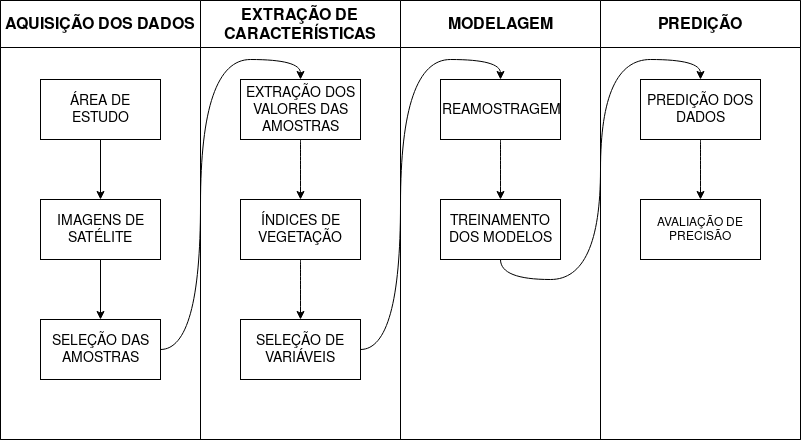
\includegraphics[scale=0.55]{figs/etapas.png}
    \legend{Fonte: Elaborado pelo autor}
\end{figure}


\chapter{Desenvolvimento}\label{desenvolvimento}

\section{Etapas}\label{etapas}

\subsection{Aquisição dos dados}\label{aquisicao-dos-dados}

\subsubsection{Área de Estudo}\label{area-de-estudo}

Primeiro, feito o \emph{download} de um arquivo no
formato \emph{shapefile}, da malha territorial do estado de São Paulo,
com divisão por município, disponibilizado pelo \sigla{IBGE}{Instituto Brasileiro de Geografia e Estatística} \cite{ibge-malha}. A partir desse arquivo, foi selecionado apenas o polígono que representa o município de Bauru. A biblioteca no R utilizada para tal operação foi a \textit{sf} \cite{sf}.

\subsubsection{Imagens de Satélite}\label{imagens-de-satelite}

Os dados do sensor Sentinel-2/MSI podem ser obtidos gratuitamente, mediante apenas a um cadastro realizado no \textit{Copernicus Open Access Hub} \cite{sentinel-data}. No R, há diversas bibliotecas que fazem a interface com a API do \textit{hub}, para este trabalho foi escholhida a \textit{getSpatialData} \cite{getSpatialData}. 
    
    O sensor multiespectral do Sentinel-2 possui as seguintes características:

\begin{table}[ht]
\centering
\caption{Características das bandas do sensor multiespectral MSI do Satélite Sentinel-2}
\begin{tabular}{rllrr}
  \hline
 banda & nome & lambda & resolucao \\ 
  \hline
 B1 & Aerosol & 0.44 &  60 \\ 
 B2 & Azul & 0.49 &  10 \\ 
 B3 & Verde & 0.56 &  10 \\ 
 B4 & Vermelho & 0.67 &  10 \\ 
 B8 & NIR & 0.84 &  10 \\ 
 B5 & Red edge 1 & 0.70 &  20 \\ 
 B6 & Red edge 2 & 0.74 &  20 \\ 
 B7 & Red edge 3 & 0.78 &  20 \\ 
 B9 & Vapor d’água & 0.94 &  60 \\ 
 B10 & Cirrus & 1.38 &  60 \\ 
 B11 & SWIR 1 & 1.61 &  20 \\ 
 B12 & SWIR 2 & 2.19 &  20 \\ 
 B8A & Red edge 4 & 0.86 &  20 \\ 
   \hline
\end{tabular}
\label{t.sentinel-msi}
\end{table}

A partir dos filtros por data e cobertura de nuvem, foram selecionadas duas imagens e então realizada uma composição entre elas para que recobrissem a área de interesse completamente. Posteriormente, foi feito um redimensionamento das bandas de 20m para 10m, para que fossem compiladas em uma única pilha de \textit{raster}. Selecionando as bandas B04, B03 E B02, é possível visualizar a imagem nas cores vermelho, verde e azul, respectivamente. A biblioteca utilizada que manipula arquivos \textit{raster} no R é a \textit{raster} \cite{raster}.

% \begin{figure}[htbp]
\begin{figure}[H]
    \centering
    \caption{Composição com as bandas vermelha, verde e azul do Sentinel-2/MSI para a região da região do município de bauru} \label{fig-fluxograma}
    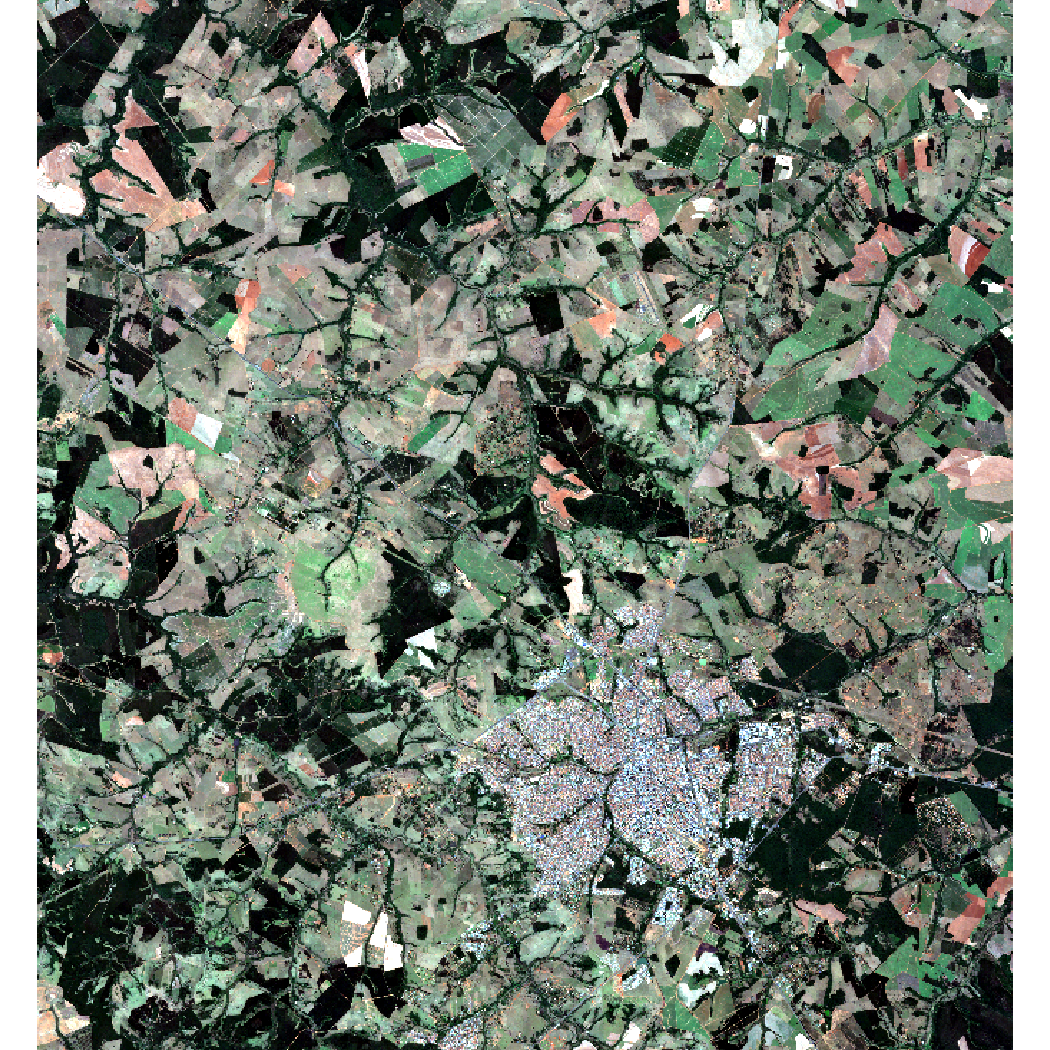
\includegraphics[scale=0.55]{figs/plot_sentinel-rgb.pdf}
    \legend{Fonte: Elaborado pelo autor}
\end{figure}

\subsubsection{Seleção de Amostras}\label{selecao-de-amostras}

    Para a seleção das amostras de treinamento, era preciso que os dados
representassem bem as classes de uso e cobertura do solo dentro do
município. De acordo com o \cite{plano-mata-atlantica} e \cite{cavassan2013bauru}, as principais unidades fitogeográficas que ocorrem no município de bauru são as formações de Floresta Estacional Semidecidual e de Cerrado, apesar de a cobertura primitiva já tenha sido muito reduzida, assim como o Cerrado no estado de São Paulo, que já representou uma área maior.

    Portanto, duas decisões foram tomadas: as amostras de treinamento
seriam provindas do bioma Cerrado; como a extensão o Cerrado é grande, a
fim de viabilizar o processamento, apenas a região de cerrado dentro do
estado de São Paulo foi selecionada.

	Para isso, foi utilizado um \textit{raster} da coleção 3.1 do projeto MapBiomas \cite{mapbiomas2018coleccao} contendo os valores de cada classe para cada pixel, definidos pela metodologia aplicada pelo projeto.

\begin{table}[H]
\centering
\caption{Classes de uso e cobertura da terra da coleção 3.1 do MapBiomas para o bioma Cerrado}
\begin{tabular}{rrl}
  \hline
 value & name.full \\ 
  \hline
 3 &         1.1.1. Formação Florestal \\ 
4 &         1.1.2. Formação Savanica \\ 
   9 &     1.2. Floresta Plantada \\ 
  12 &     2.2. Formação Campestre \\ 
  15 &     3.1. Pastagem \\ 
  19 &          3.2.1. Cultura Anual e Perene \\ 
  20 &          3.2.2. Cultura Semi-Perene \\ 
  21 &     3.3. Mosaico de Agricultura e Pastagem \\ 
  24 &     4.2. Infraestrutura Urbana \\ 
  33 &     5.1 Rio, Lago e Oceano \\ 
   \hline
\end{tabular}
\end{table}

    Esse \emph{raster} foi recortado para o tamanho do polígono do estado
de São Paulo. Em seguida, foi feito a seleção de 200 amostras aleatórias
de cada classe, e exportado para um arquivo \emph{shapefile}.

\begin{figure}[H]
    \centering
    \caption{Amostras aleatórias de pontos para }
    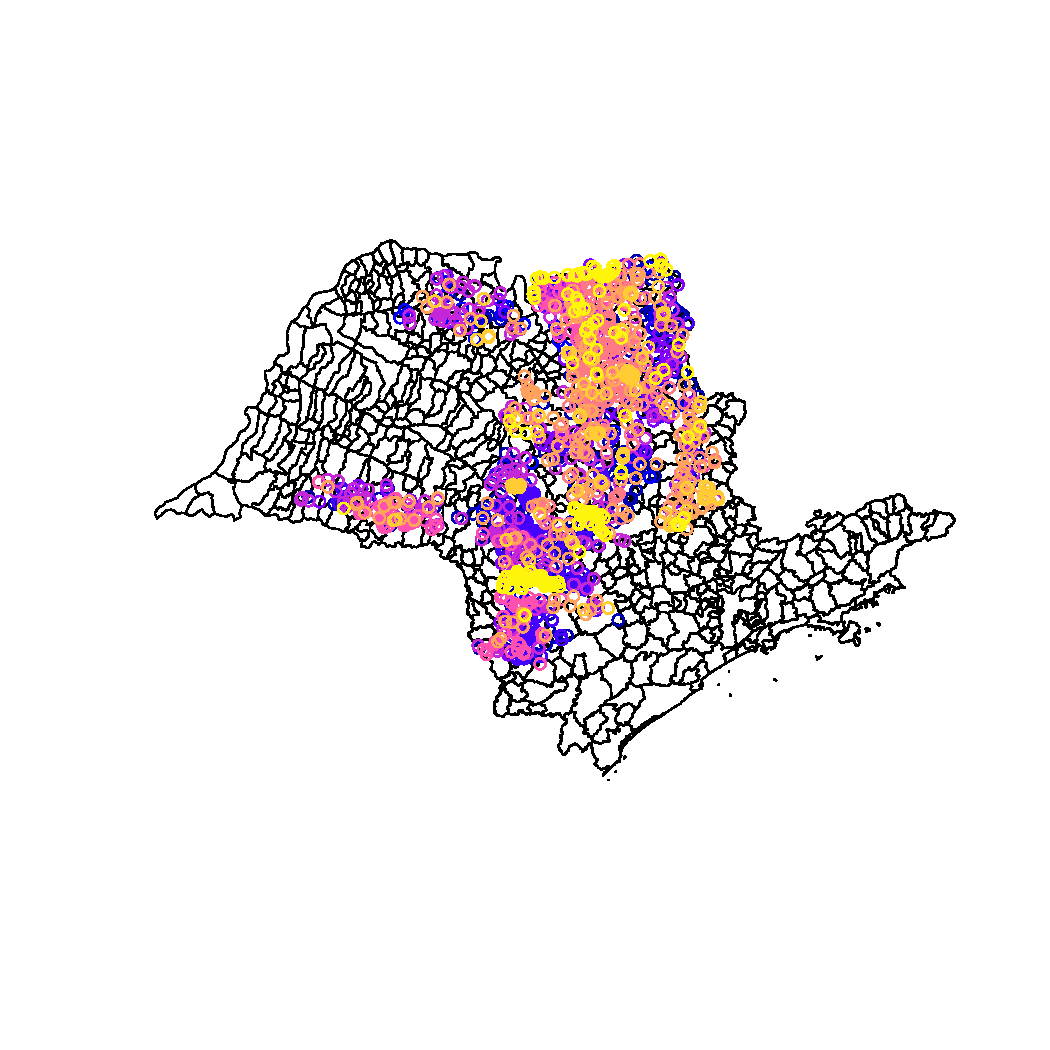
\includegraphics[scale=0.6]{figs/plot_pontos-amostra.pdf}
    \legend{Fonte: Elaborado pelo autor}
\end{figure}

\subsection{Extração de
Características}\label{extracao-de-caracteristicas}

	A etapa da extração de características envolve a seleção das variáveis
usadas no processo de classificação, que podem ser as assinaturas
espectrais das bandas, índices de vegetação, informação de textura,
entre outras \cite{lu-weng}

\subsubsection{Extração dos Valores das
Amostras}\label{extracao-dos-valores-das-amostras}

    A próxima etapa, foi a de extração dos valores das amostras. Cada
coordenada gerada na última etapa, contém a informação da classe que ela representa, então o próximo passo foi de extrair os valores de cada
banda naquele ponto, e então compor a tabela com as variáveis preditoras
para a modelagem de aprendizado de máquina.

    Nessa etapa, foi utilizado o ambiente do \textit{Google Earth Engine} \cite{gorelick2017google} , onde o \emph{shapefile} foi carregado, foi feita uma composição com imagens do satélite Sentinel-2, filtradas por baixa porcentagem de nuvens e para a região em que os pontos estão compreendidos. Em seguida, para cada ponto, foi extraído os valores das bandas e exportado para um arquivo \emph{geojson}, que foi importado de volta ao ambiente do RStudio.
    
\begin{table}[H]
    \caption{Quantidade de exemplos de treinamento para cada classe}
  	\centering
  	\begin{tabular}{rlr}
    	\hline
   		& Classes & Frequência \\ 
    	\hline
  	1 & agricultura\_pastagem & 197 \\ 
    2 & cultura\_anual\_perene & 146 \\ 
    3 & cultura\_semi\_perene & 200 \\ 
    4 & floresta\_plantada & 200 \\ 
    5 & formacao\_campestre & 140 \\ 
    6 & formacao\_florestal & 199 \\ 
    7 & formacao\_savanica &  91 \\ 
    8 & infra\_urbana & 105 \\ 
    9 & pastagem & 198 \\ 
    10 & rio\_lago\_oceano & 159 \\ 
    	\hline
	\end{tabular}
\end{table}

É importante notar que para algumas classes, na execução da amostragem, foram selecionados menos do que 200 amostras. 

    Em um sistema de classificação, antes da extração dos valores dos pontos das amostras, seria interessante que a imagem passasse por um
processo de pré processamento. Essa etapa incluiria a aplicação de
técnicas de processamento de imagens para correções atmosféricas e
geométricas, eliminação de ruídos, entre outras \cite{lu-weng}. Contudo, uma característica das imagens do Sentinel-2/MSI, é de que há uma série de etapas de pré processamento, como as mencionadas, que são realizadas antes das imagens serem disponibilizadas. 

\subsubsection{Índices de
Vegetação}\label{indices-de-vegetacao}

	Os índices de vegetação são obtidos através de operações aritméticas
entre as bandas. Possuem a característica de realçar as variações de
densidade da cobertura vegetal \cite{meneses2012introduccao}. O NDVI é provavelmente o mais utilizado, ou pelo menos o mais conhecido. Esse índice possui a característica de evidenciar áreas da vegetação fotossinteticamente mais ativas. O cálculo do NDVI, que varia de 0 a 1, é dado por: 

\begin{equation}
NDVI = \frac{NIR - RED}{NIR + RED}
\end{equation}

Onde $NIR$ é o valor para a banda na região do infravermelho próximo
(a banda 8 do Sentinel-2/MSI) e $RED$ é a banda na região do vermelho (banda 4).

\begin{figure}[H]
    \centering
    \caption{Representação do cálculo do índice NDVI} \label{fig-fluxograma}
    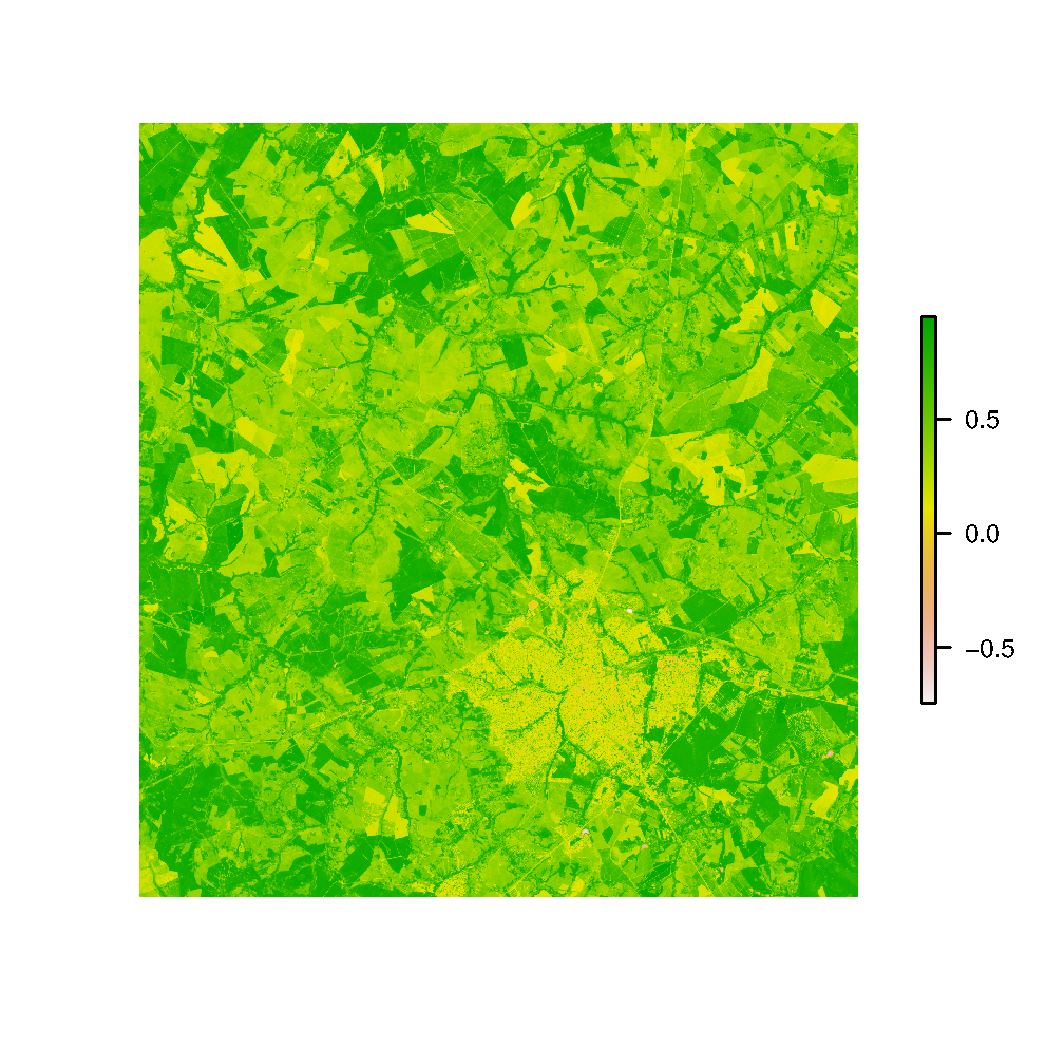
\includegraphics[scale=0.7]{figs/plot_ndvi.pdf}
    \legend{Fonte: Elaborado pelo autor}
\end{figure}

\subsubsection{Seleção de Variáveis}\label{selecao-de-variaveis}

	Como variáveis preditoras, foram selecionadas as bandas ``SWIR1'',
``SWIR2'', ``Azul'', ``Verde'', ``Vermelho'', ``NIR'', ``RE1'', ``RE2'',
``RE3'', ``RE4'' e uma nova coluna contendo o cálculo do NDVI para cada
ponto da amostra.


\subsection{Modelagem}\label{modelagem}

	O pacote \emph{caret} (\emph{Classification And REgression Training}) \cite{caret} R contém funções para otimizar o processo de treinamento de modelos para problemas de regressão e classificação. Ele funciona como um agregador de diversos pacotes que contém métodos de aprendizado estatístico, fazendo a interface entre as funções disponíveis no pacote para controle do processo de treinamento e avaliação de resultados.

\subsubsection{Reamostragem}\label{reamostragem}

	A primeira etapa para a criação dos modelos, foi a divisão do conjunto
de dados em dois subconjuntos: um de treinamento (75\%) e outro de teste (25\%). Utilizando a função de validação cruzada do \emph{caret}, na criação do modelo, o conjunto de treinamento é reparticionado em 10, e então, a partir dessa repetições no ajuste, é escolhido o conjunto de
parâmetros que teve melhor resultado para aquele método.

\subsubsection{Treinamento}\label{treinamento}

	Na etapa do treinamento dos modelos, para a seleção dos parâmetros
utilizados em cada algoritmo foi utilizada a técnica da validação
cruzada \emph{k-fold} (não é o mesmo que na última etapa), onde os dados de treinamento são subdivididos em \emph{k} subconjuntos e então, o modelo é calculado \emph{k} vezes, e então, o resultado é comparado para seleção do parâmetro (ou conjunto) que obteve melhor resultado, no caso, o método de comparação utilizado foi a acurácia geral a partir da matriz de confusão gerada para cada modelo.

	O primeiro modelo foi treinado com o algoritmo MVS (\emph{svmRadial} no \emph{caret}), utilizado como núcleo a função de base radial dada por: 
    \begin{equation}
	K(x,y) = \exp(-\frac{\parallel x-y^{2} \parallel}{\sigma^{2}})    
    \end{equation}
	Após o treinamento do modelo, foram selecionados os parâmetros $C = 1$ e $Sigma = 1$.
    
\begin{figure}[H]
    \centering
    \caption{Parâmetros selecionados após treinamento com o algoritmo maquina de vetores suporte com núcleo radial} \label{fig-fluxograma}
    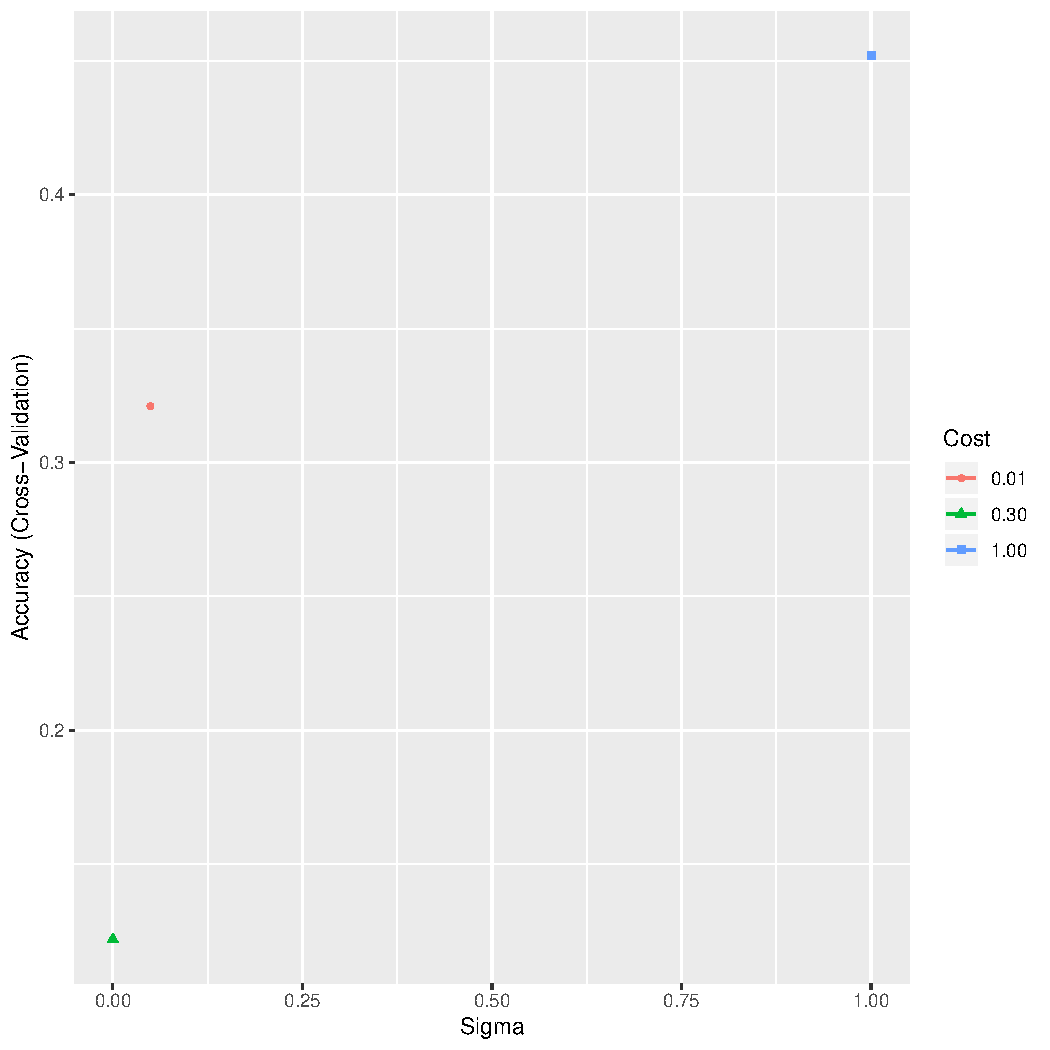
\includegraphics[scale=0.5]{figs/plot_svm-radial.pdf}
    \legend{Fonte: Elaborado pelo autor}
\end{figure}

	O próximo modelo, foi MVS também, porém linear (\emph{svmLinear3} no
\emph{caret}), ou seja, sem função de núcleo e com regularização, que
significa aplicar um custo de penalização nos parâmetros $\theta$. Os
parâmetros selecionados foram C = 0.03 e Loss = L2.

\begin{figure}[H]
    \centering
    \caption{Parâmetros selecionados após treinamento com o algoritmo maquina de vetores suporte linear com regularização} \label{fig-fluxograma}
    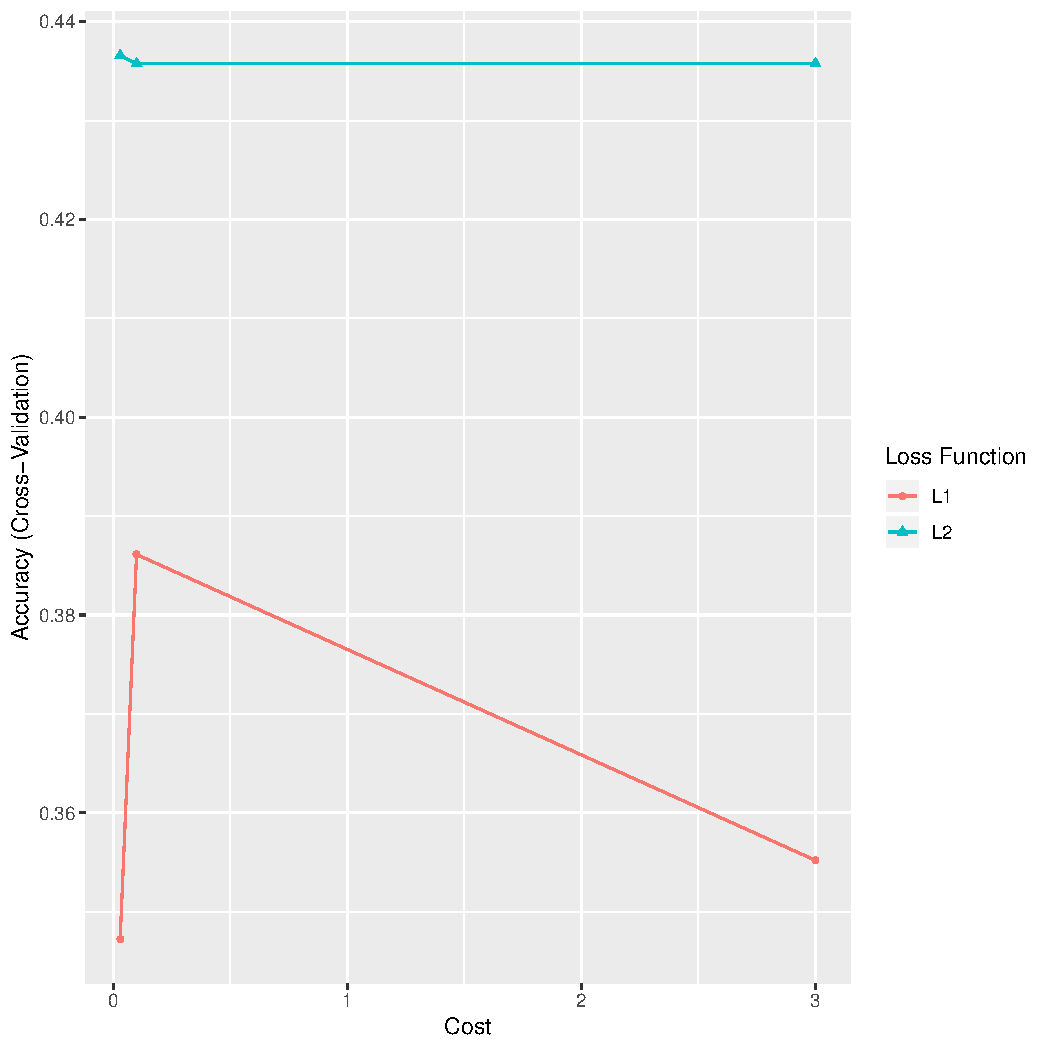
\includegraphics[scale=0.5]{figs/plot_svm-linear.pdf}
    \legend{Fonte: Elaborado pelo autor}
\end{figure}

	Por último, foi computado também um modelo utilizando Florestas
Aleatórias (\emph{rf} no \emph{caret}), com o parâmetro selecionado mtry
= 3.

\begin{figure}[H]
    \centering
    \caption{Parâmetros selecionados após treinamento com o algoritmo florestas aleatórias} 
    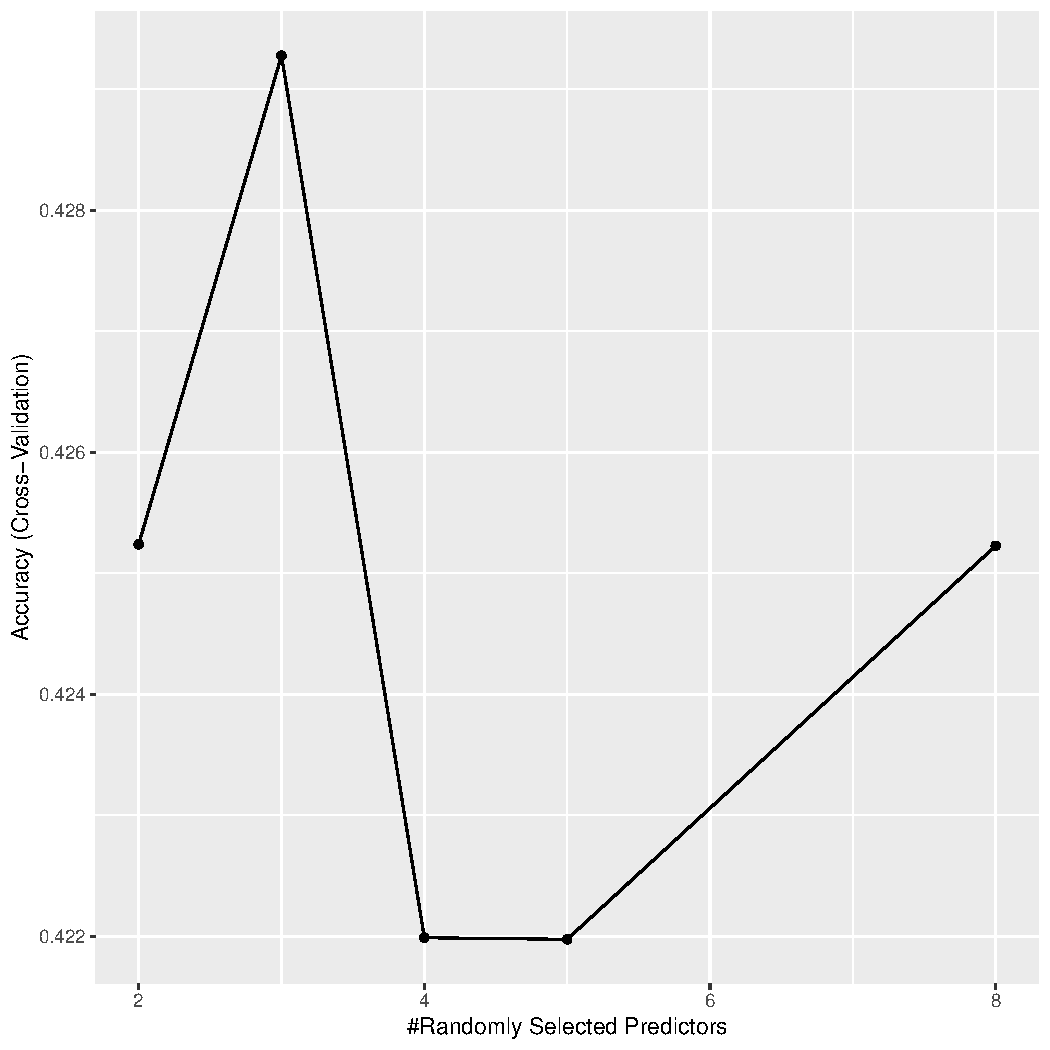
\includegraphics[scale=0.5]{figs/plot_rf.pdf}
    \legend{Fonte: Elaborado pelo autor}
\end{figure}

\section{Resultados}\label{resultados}

\subsection{Predição dos Dados}\label{predicao-dos-dados}

	Para cada modelo treinado, foi realizada uma predição com a imagem
selecionada anteriormente do sensor  Sentinel-2/MSI para a região do
município de Bauru, resultando em \emph{rasters} com os valores para
cada classes usadas para a criação dos modelos, demonstrados a seguir:

\begin{figure}[H]
    \centering
    \caption{Mapa com classes de uso e cobertura da terra obtido a partir da predição do modelo utilizando máquina de vetores suporte com núcleo radial} 
    \includegraphics[scale=0.8]{figs/map_svm-radial.pdf}
    \legend{Fonte: Elaborado pelo autor}
\end{figure}
\begin{figure}[H]
    \centering
    \caption{Mapa com classes de uso e cobertura da terra obtido a partir da predição do modelo utilizando máquina de vetores suporte linear com regularização} 
    \includegraphics[scale=0.8]{figs/map_svm-linear.pdf}
    \legend{Fonte: Elaborado pelo autor}
\end{figure}
\begin{figure}[H]
    \centering
    \caption{Mapa com classes de uso e cobertura da terra obtido a partir da predição do modelo utilizando florestas aleatórias} 
    \includegraphics[scale=0.8]{figs/map_rf.pdf}
    \legend{Fonte: Elaborado pelo autor}
\end{figure}

\subsubsection{Avaliação de
Precisão}\label{avaliacao-de-precisao}

Para a avaliação da qualidade das predições realizadas, foi computado
a matriz de confusão de cada uma, a partir dos índices calculados a
partir da matriz de erro. A matriz de erro por sua vez foi montada a
partir da seleção de 100 pontos de amostras para cada classe dos
\emph{rasters} obtidos na etapa da predição, e em seguida, os valores
dos pontos foram extraídos de um conjunto verdade, que é um
\emph{raster} da mesma região com a classificação realizada pela
iniciativa MapBiomas e disponibilizada para download. Para comparação
visual com os mapas apresentados anteriormente, o \emph{raster} do
MapBiomas está representado a seguir:

\begin{figure}[H]
    \centering
    \caption{Mapa com classes de uso e cobertura da terra obtido a partir da classificação realizada pela iniciativa MapBiomas} 
    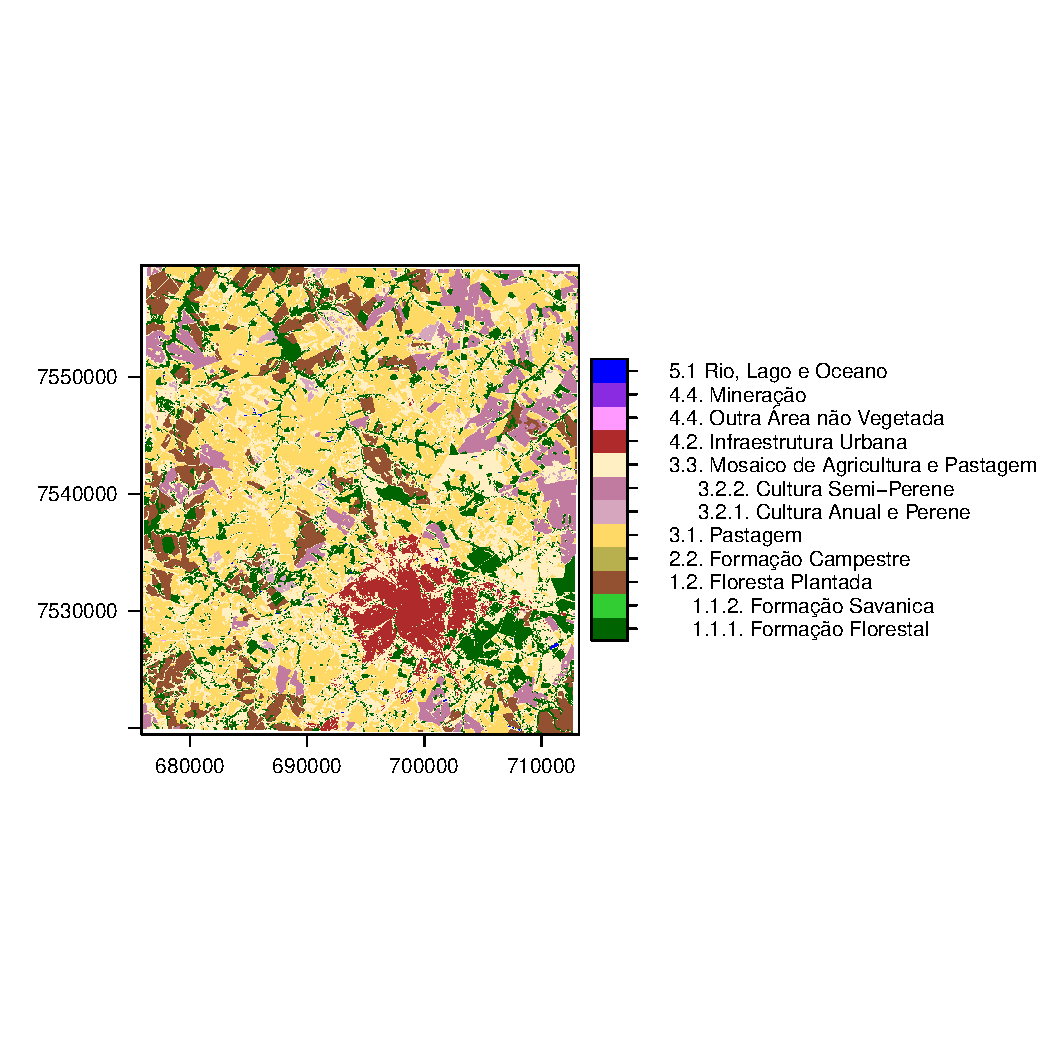
\includegraphics[scale=0.8]{figs/map_mapbiomas.pdf}
    \legend{Fonte: Elaborado pelo autor}
\end{figure}

Com destaque para os índices \emph{kappa} e \emph{accuracy} (acurácia geral), na tabela a seguir estão demonstrados os valores dos resultados:

\begin{table}[H]
\caption{Tabela de avaliação de precisão das predições realizadas}
\centering
\begin{tabular}{rlrr}
  \hline
 & Modelo & Kappa & Acuracia \\ 
  \hline
1 & MVS linear & 0.30 & 0.38 \\ 
  2 & MVS radial & 0.27 & 0.39 \\ 
  3 & Florestas Aleatorias & 0.13 & 0.23 \\ 
   \hline
\end{tabular}
\end{table}

\subsubsection{Considerações}\label{considerauxe7uxf5es}

Comparando visualmente os mapas obtidos com o mapa do MapBiomas além da matriz de erro gerada, pôde-se notar algumas classes que sofreram certa confusão, como é o caso da \emph{formação\_florestal} na predição com FA, que na verdade representariam a classe \emph{floresta\_plantada}. Levando em consideração que na  metodologia do MapBiomas aplicada nos dados de
treinamento são utilizadas outras variáveis de predição (como outros
índices de vegetação), é provável que apenas as bandas selecionadas e o
NDVI não seja suficiente para separar com precisão todas as classes
utilizadas, como \cite{lu-weng} apontam no artigo o qual este trabalho se
baseou. Ainda no caso dessa predição, a acurácia foi prejudicada pelo
fato dos \emph{pixels} apresentarem pouca homogeneidade nos espaços
vizinhos. A predição realizada com o algoritmo MVS com núcleo não
linear, apesar de apresentar uma acurácia mediana, resultou em poucas
classes que predominaram. A classificação que obteve melhor resultado
foi a que utilizou MVS linear para criação do modelo.

\chapter{Conclusão}\label{conclusuxe3o}

    O estudo de metodologias de análise e inferência de dados gerados a
partir da Observação da Terra permite que seja realizado o monitoramento
dos recursos terrestres. A característica dos sistemas de Sensoriamento
Remoto permite o imageamento da superfície terrestre em escala global e
de maneira frequente. Nesse contexto, métodos de classificação de
imagens digitais tornam-se essenciais para extração de dados que poderão
ser usados em outros estudos de diversas áreas.

    Além disso, atualmente, plataformas baseadas em nuvem - que computam
os dados em servidores remotos e com alta capacidade de processamento -
viabilizam a coleta, distribuição e processamento de dados coletados por
Sensoriamento Remoto. Com a utilização das imagens de satélite
distribuídas gratuitamente bem como as ferramentas e \emph{softwares}
livres disponíveis, juntamente (porém de maneira opcional) com as
plataformas de nuvem, as aplicações tornam-se acessíveis.

    Métodos de classificação a partir de aprendizado de máquina vêm sendo
amplamente utilizados em diversas áreas do conhecimento. Em
Sensoriamento Remoto, esses métodos são interessantes por fazerem pouca
ou nenhuma suposição dos dados e dão bons resultados. Neste trabalho,
foi realizado um estudo de um processo de classificação, passando pela
aquisição dos dados, extração de características, modelagem e por fim,
avaliação de precisão.

    Pôde-se perceber como cada uma das etapas exige uma série de
considerações precisam ser avaliadas para se obterem bons resultados, e
muitas delas exigem conhecimento especializado. Portanto, como resultado
final, este trabalho não alcançou todos os objetivos propostos de
maneira satisfatória.

\section{Trabalhos Futuros}\label{trabalhos-futuros}

    A partir de um modelo preditivo bem ajustado, uma aplicação
interessante é a análise temporal de uma região de interesse, a partir
da comparação das alterações nas classes ao longo de um determinado
período. Outras aplicações podem ser por exemplo: planejamento urbano,
monitoramento ambiental, cruzamento com outros dados, entre outras. No
escopo deste trabalho, alguns ajustes e aprofundamento nas etapas também
podem ser realizados como por exemplo: utilização de outros dados que
não os do MapBiomas, a fim de comparação; seleção de amostras de outras
regiões; etapas adicionais de pré processamento para extração de valores
das amostras de treinamento; extração de outras características, como
outros índices; utilização de outros algoritmos como Redes Neurais para
comparação.



%\chapter{Introdução}
\label{c.introducao}

Para iniciar a produção em .tex é necessário instalar os pacotes básicos da linguagem e seus compiladores. O MiKTeX é um pacote básico para o Windows (miktex.org/download) e o MacTeX um pacote básico para o Mac (tug.org/mactex) que contém o mínimo necessário de TeX/LaTeX para rodar. Ele já vem com os compiladores nativos da linguagem e uma IDE (TeXworks, para edição do texto) que possui o compilador integrado.

Normalmente é utilizado o modo pdfLaTeX + MakeIndex + BibTeX para compilar um arquivo .tex. Existem outros formatos de compiladores, mas essa opção é capaz de gerar um .pdf automático após a compilação e ainda por cima adicionar as funcionalidades do BibTeX (recursos para criação e montagem automática de fontes bibliográficas).

Além disso, também é necessária a instalação do pacote abnTeX2. Esse tutorial \url{https://github.com/abntex/abntex2/wiki/Instalacao} provém o passo a passo de como instalar cada componente do TeX, em qualquer sistema operacional (Linux, Mac OS e Windows). Caso esteja utilizando o MiKTeX, ele é capaz de efetuar o download do pacote automaticamente, apenas instale-o, abra o projeto.tex e compile-o, ele irá requisitar a autorização para baixar automaticamente os pacotes que faltam para efetuar a compilação.

Com tudo em mãos e o compilador funcionando, é hora de abrir o modelo (projeto.tex) e começar a escrever o texto. É possível perceber no código a estrutura do arquivo e os campos possíveis de edição. Ao escrever o texto, ele é escrito normalmente, sendo que existem diversos comandos para estilizá-lo, criar tabelas, figuras, dentre outros. A seguir abordaremos os principais comandos e funções que podem ser utilizadas em um projeto básico de TCC. Para outras funções e pacotes, procure no Google, a comunidade é ativa e provavelmente já deve ter feito o que é de sua necessidade.

O arquivo projeto.tex contém os pacotes e comandos básicos que definem a estrutura desse texto já no formato requisitado pela ABNT. Dentro dele é possível ver que estamos importando outros dois arquivos .tex (introducao e conclusao), ou seja, esses arquivos estão sendo basicamente concatenados com o comando ``input''. A divisão não é necessária, mas pode ser que auxilie na escrita do texto  ao deixar as coisas mais separadas e organizadas, não sendo um único arquivo cheio de linhas e linhas de código.

\section{Modificadores de Texto}
\label{s.modificador}

Os modificadores de texto mais simples utilizados são o negrito (``textbf'') \textbf{texto em negrito} e o itálico (``emph'') \emph{texto em itálico}.

\section{Seções}
\label{s.citacoes}

Seções podem ser criadas a partir do comando ``section'' e hierarquizadas abaixo do capítulo principal. É possível referenciá-las, por exemplo, Seção~\ref{s.citacoes} corresponde a seção atual em que estamos. Já se quisermos referenciar alguma outra coisa, é só utilizarmos o comando ``ref'' presente no código desse texto, por exemplo, Capítulo~\ref{c.introducao}.

\subsection{Subseções}
\label{ss.subsecao}

Subseções também podem ser criadas com o comando ``subsection'' e referenciadas~\ref{ss.subsecao}.

\subsubsection{Sub-subseções}
\label{sss.subsubsecao}

Também há mais um nível que pode ser criado com o comando ``subsubsection''.

\section{Alíneas}
\label{s.alineas}

\begin{alineas}

\item As alineas devem ser criadas desse modo, com o comando begin\{alineas\}. Isso é necessário para que estejam no formato definido pelo pacote abnTeX2 e, consequentemente, no formato definido pela ABNT.

\item Cada item da alínea pode ser invocado com um comando item.

\item O fim de cada alínea é determinado por end\{alineas\}.

\end{alineas}

\section{Tabelas}
\label{s.tabelas}

As tabelas também podem ser referenciadas como se fossem seções ou figuras, por exemplo, esta é a Tabela~\ref{t.transacao-mercado}.

\begin{table}[htb]
\centering
\caption{Exemplo de transações de mercado.}
\begin{tabular}{c|c}
\hline
\textbf{\small TID} & \textbf{\small Conjunto de Itens}\\\hline \hline
{\small 1} & {\small \{Pão, Leite\}}\\\hline
{\small 2} & {\small \{Pão, Fralda, Cerveja, Ovos\}}\\\hline
{\small 3} & {\small \{Leite, Fralda, Cerveja, Coca-Cola\}}\\\hline
{\small 4} & {\small \{Pão, Leite, Fralda, Cerveja\}}\\\hline
{\small 5} & {\small \{Pão, Leite, Fralda, Coca-Cola\}}\\\hline
\end{tabular}
\label{t.transacao-mercado}
\end{table}

Quando uma tabela é criada com begin\{table\}, ela é automaticamente adicionada à Lista de Tabelas.

\section{Quadros}

Este modelo vem com o ambiente \texttt{quadro} e impressão de Lista de quadros 
configurados por padrão. Verifique um exemplo de utilização:

\begin{quadro}[htb]
\caption{\label{quadro-exemplo}Exemplo de quadro}
\begin{tabular}{|c|c|c|c|}
	\hline
	\textbf{Pessoa} & \textbf{Idade} & \textbf{Peso} & \textbf{Altura} \\ \hline
	Marcos & 26    & 68   & 178    \\ \hline
	Ivone  & 22    & 57   & 162    \\ \hline
	...    & ...   & ...  & ...    \\ \hline
	Sueli  & 40    & 65   & 153    \\ \hline
\end{tabular}
\fonte{Autor.}
\end{quadro}

Este parágrafo apresenta como referenciar o quadro no texto, requisito
obrigatório da ABNT. 
Primeira opção, utilizando \texttt{autoref}: Ver o \autoref{quadro-exemplo}. 
Segunda opção, utilizando  \texttt{ref}: Ver o Quadro \ref{quadro-exemplo}.



\section{Algoritmos}
\label{s.algoritmos}

O pacote nicealgo incluído nos arquivos desse projeto é responsável por disponibilizar comandos extras, não inerentes ao básico TeX, para a criação de algoritmos. Um exemplo do Algoritmo~\ref{a.algoritmo} é escrito a seguir. Eles também pode ser referenciados como se fossem tabelas ou figuras.


\par
\needspace{20\baselineskip}

\begin{nicealgo}{a.algoritmo}
\naTITLE{Algoritmo AIS}
\naPREAMBLE
\naINPUT{Conjunto Frequente L = 0 e Grupo de Fronteira F = 0.}
\naBODY
\naBEGIN{\textbf{Enquanto} $F \neq 0$, \textbf{faça}}
\na{\textbf{Seja} conjunto candidato $C = 0$;}
\naBEGIN{\textbf{Para cada} tuplas $t$ da base de dados, \textbf{faça}}
\naBEGIN{\textbf{Para cada} conjuntos de itens $f$ em $F$, \textbf{faça}}
\naBEGIN{\textbf{Se} $t$ contém $f$, \textbf{então}}
\naEND{\textbf{Seja} $C_f =$ conjuntos de itens candidatos extensões de $f$ e contidos em $t$;}
\naBEGIN{\textbf{Para cada} conjunto de itens $c_f$ em $C_f$, \textbf{faça}}
\naBEGIN{\textbf{Se} $c_f \in C$, \textbf{então}}
\naEND{$c_f$.contagem $= c_f$.contagem$ + 1$;}
\naBEGIN{\textbf{Se não}}
\na{$c_f$.contagem $= 0$;}
\naEND{$C = C + c_f$;}
\naEND{}
\naEND{}
\naEND{}
\na{\textbf{Seja} F = 0;}
\naBEGIN{\textbf{Para cada} conjunto de itens $c$ em $C$, \textbf{faça}}
\naBEGIN{\textbf{Se} $contagem(c)/tamanho\_db > minsupport$, \textbf{então}}
\naEND{$L = L + c$;}
\naBEGIN{\textbf{Se} $c$ deve ser usado como a próxima fronteira, \textbf{então}}
\naEND{$F = F + c$;}
\naEND{}
\naEND{}
\end{nicealgo}


\section{Códigos}
\label{s.codigos}

Códigos podem ser criados a partir do comando begin\{lstlisting\} e end\{lstlisting\}. É possível passar parâmetros para essa função, como por exemplo, a linguage do código e a legenda dele. Por exemplo: \char`\\begin\{lstlisting\}[language=Python, caption=Exemplo de código em Python]

\begin{lstlisting}[language=Python, caption=Exemplo de código em Python]
import numpy as np
 
def incmatrix(genl1,genl2):
    m = len(genl1)
    n = len(genl2)
    M = None #to become the incidence matrix
    VT = np.zeros((n*m,1), int)  #dummy variable
 
    #compute the bitwise xor matrix
    M1 = bitxormatrix(genl1)
    M2 = np.triu(bitxormatrix(genl2),1) 
 
    for i in range(m-1):
        for j in range(i+1, m):
            [r,c] = np.where(M2 == M1[i,j])
            for k in range(len(r)):
                VT[(i)*n + r[k]] = 1;
                VT[(i)*n + c[k]] = 1;
                VT[(j)*n + r[k]] = 1;
                VT[(j)*n + c[k]] = 1;
 
                if M is None:
                    M = np.copy(VT)
                else:
                    M = np.concatenate((M, VT), 1)
 
                VT = np.zeros((n*m,1), int)
 
    return M
\end{lstlisting}


\section{Figuras}
\label{s.figuras}

Este parágrafo apresenta como referenciar figura no texto, requisito obrigatório da ABNT.
Primeira opção, utilizando \texttt{autoref}: Ver a \autoref{f.disposicao-mercado}. 
Segunda opção, utilizando  \texttt{ref}: Ver a Figura \ref{f.disposicao-mercado}.

Atente-se ao código para perceber um possível redimensionamento com a função scale e o caminho de onde a figura deve ser retirada.

Quando uma figura é criada com begin\{figure\}, ela é automaticamente adicionada à Lista de Ilustrações.

\begin{figure}[htbp]
\caption{\small Exemplo do ambiente TeXworks.}
\centering
\includegraphics[scale=0.50]{figs/tex-exemplo.png}
\label{f.disposicao-mercado}
\legend{\small Fonte: Elaborada pelo autor.}
\end{figure}

\begin{figure}[htbp]
    \centering
    \caption{Imagem 1 da minipage} \label{fig-minipage-imagem1}
    \includegraphics[scale=0.9]{figs/abntex2-modelo-img-marca.pdf}
    \legend{Fonte: Produzido pelos autores}
\end{figure}


\section{Equações}
\label{s.equacoes}

O TeX também é muito famoso pela forma em que consegue tratar funções e símbolos matemáticos. A partir da utiização de dois cifrões (\$codigo matemático\$) é possível identificar ao compilador que a escrita a seguir são símbolos e códigos originários do pacote matemático do TeX. Aqui estamos demonstrado um exemplo $\phi = 1 + x$ dessa utilização.

Também podemos definir equações utilizando os comandos begin\{equation\} e end\{equation\}. Por exemplo:

\begin{equation}
\label{e.energy-rbm}
E(\textbf{v},\textbf{h})=-\sum_{i=1}^ma_iv_i-\sum_{j=1}^nb_jh_j-\sum_{i=1}^m\sum_{j=1}^nv_ih_jw_{ij},
\end{equation}

\begin{equation}
\label{e.probability-configuration}
P(\textbf{v},\textbf{h})=\frac{e^{-E(\textbf{v},\textbf{h})}}{\displaystyle\sum_{\textbf{v},\textbf{h}}e^{-E(\textbf{v},\textbf{h})}},
\end{equation}

\begin{eqnarray}
\label{eq:par}
\hat{\phi}^j & = & \left\{ \begin{array}{ll} \hat{\phi}^j\pm \varphi_j \varrho  & \mbox{{ com probabilidade PAR}} \\
    \hat{\phi}^j & \mbox{{com probabilidade (1-PAR).}}
\end{array}\right.
\end{eqnarray}

Existem diversos sites no Google que contém códigos de símbolos e funções matemáticas de todos os tipos. Exemplo:\\
\begin{center}
\tiny estudijas.lu.lv/pluginfile.php/14809/mod\_page/content/16/instrukcijas/matematika\_moodle/LaTeX\_Symbols.pdf.
\end{center}

\section{Como citar as referências}
\label{ss.referencias}

Aqui está um exemplo de como podemos referenciar as bibliografias utilizadas no trabalho. Elas são guardadas na forma de metadados (tags) no arquivo .bib a qual é importada no projeto principal (projeto.tex).

E podemos citá-las de acordo com os identificadores atribuídos para cada referência, por exemplo,~\cite{stonebraker93} ,~\cite{rocha09} e~\cite{keras}.

Após citar um item de referência bibliográfica com o comando ``cite'', ela será automaticamente padronizada e incluída na página de Referências de seu arquivo. Atualmente os maiores sites portadores de artigos, periódicos, dentre outros (IEEE, Springer, etc) já conseguem exportar a publicação desejado no formato BibTeX, sendo facilmente adicionado ao arquivo .bib de seu trabalho.

Muitas vezes não é possível exportar publicações diretamente para o formato BibTeX, como, por exemplo, na citação de sites. Para mais informações sobre como criar manualmente arquivos BibTeX: \url{https://github.com/abntex/limarka/wiki/Adicionando-refer%C3%AAncias}

%\section{Entrada de Siglas e Símbolos}
%Quando uma sigla ou símbolo são criados com os comandos abaixo, elas são automaticamente adicionadas à Lista de abreviaturas/siglas ou Lista de símbolos.
%
%\sigla{ABNT}{Associação Brasileira de Normas Técnicas}, 
%
%De acordo com \acs{ABNT}...
%
%\sigla{SUPRE-MISS}{Suicide Prevention Multisite Intervention Study on Suicidal Behaviors}
%
%\sigla{SIRGAS2000}{Sistema de referência geocêntrico para as américas época 2000.4}
%
%\sigla{UNESP}{Universidade Estadual Paulista "Júlio de Mesquita Filho" }
%
%\sigla{ONU}{Organição Nacional da União}
%
%\sigla{abnTeX}{ABsurdas Normas para TeX}
%
%\simbolo{gama}{$ \Gamma $}{Letra grega Gama}, \simbolo{lambda}{$ \Lambda $}{Lambda}
%
%\simbolo{zeta}{$ \zeta $}{Letra grega minúscula zeta}
%
%\simbolo{pertence}{$ \in $}{Pertence}
% 
%\simbolo{pi}{$ \pi $}{Número pi}
%
%A constante \gls{pi}... 
 
\section{Notas}
\begin{itemize}
    \item O título de quadros e tabelas são sempre em cima.
    \item Sempre que possível, utilize o comando autoref.
    \item todas as figuras da monografia precisam estar referenciadas no texto pelo menos uma vez.
\end{itemize}
%\chapter{Fundamentação Teórica}
\label{c.fundamentacao}


%\chapter{Conclusão}
\label{c.conclusao}

Os arquivos estão sendo concatenados. Podemos continuar a nossa escrita em outro arquivo .tex desde que ele seja importado no projeto principal, que é sempre o utilizado para efetuar a compilação.


% --------------------------------------------------------
% ELEMENTOS PÓS-TEXTUAIS
% --------------------------------------------------------

\postextual


% --------------------------------------------------------
% REFERÊNCIAS BIBLIOGRÁFICAS
% --------------------------------------------------------

\bibliography{chapters/referencias}


% --------------------------------------------------------
% GLOSSÁRIO
% --------------------------------------------------------

% Consulte o manual da classe abntex2 para orientações sobre o glossário.
%\glossary


% --------------------------------------------------------
% APÊNDICES
% --------------------------------------------------------

% Inicia os apêndices
%\begin{apendicesenv}
% Imprime uma página indicando o início dos apêndices
%\partapendices
% Criação do apêndice
%\end{apendicesenv}


% --------------------------------------------------------
% ÍNDICE REMISSIVO
% --------------------------------------------------------

\printindex


% --------------------------------------------------------
% FINAL DO DOCUMENTO
% --------------------------------------------------------

\end{document}
